\chapter{The ancient geomagnetic field}


\noindent
BACKGROUND: 
read Kono, (2007);   \nocite{kono07} 
Merrill et al. (1996), Chapters 1, 2.4, 4, 6.4. \nocite{merrill96}

\vskip 24pt



The magnetic field is one component of the highly complex Earth system.  It interacts with the atmosphere, the biosphere,  the deep mantle and even the inner core.  It also has the useful property of pointing roughly North (or South).  Records of the Earth's magnetic field play a role in many aspects of Earth Science; hence some knowledge of how it behaves is important to all Earth scientists.   The following introduces some of the reasons for studying the geomagnetic field.   


\begin{enumerate}
\item {\it Atmospheric interaction: }
  Radioactive forms of carbon, beryllium and chlorine are produced in the atmosphere by cosmic ray bombardment.  The decay of these isotopes is used for dating purposes in a wide variety of disciplines.   There are large variations in ages predicted from tree ring, varve or ice layer counting or U/Th dating and those estimated by radiocarbon dating (see Figure~\ref{fig:c14}).  Some of these variations are caused by changes in the carbon balance between the atmosphere and the deep ocean (which is a reservoir of old carbon) and some could be caused by changes in magnetic field strength. Because the magnetic field shields the atmosphere to a large extent from cosmic rays,   changes in the intensity of the magnetic field result in changes in production, hence are
 key to  deriving accurate age information.    To date, there is rather poor agreement between the variations in radiocarbon production predicted using changes in paleointensity of the geomagnetic field (compare Figure~\ref{fig:c14}b with c.)  Either the field variations are not known, the relationship between those variations and radiocarbon production is not known or the actual variations in production are not known because of unconstrained reservoir effects (or any combination of these factors).  



\item {\it Biospheric interaction:}
 Some life forms make magnetic crystals (Figure~\ref{fig:bacteria}).   In the case of magnetotactic bacteria, these tiny magnets are used for physical orientation.  In some cases, animals may use magnetic field lines for navigation.  
 
 \begin{figure}[h!tb]
%\epsfxsize 14cm
%\centering \epsffile{EPSfiles/c14.eps}
\centering  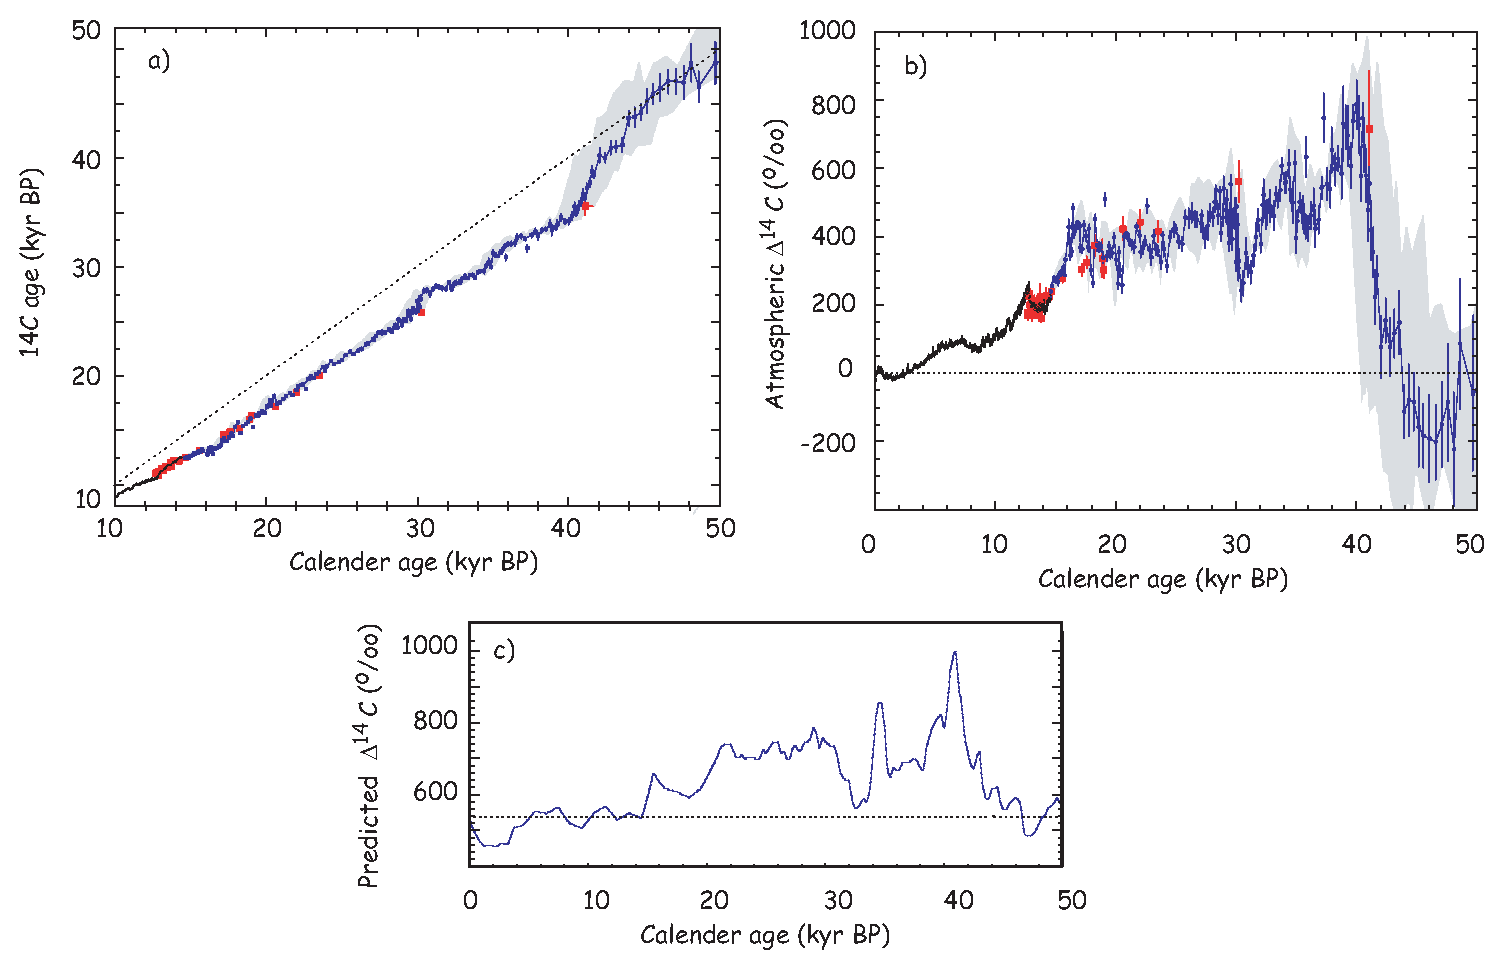
\includegraphics[width=14 cm]{EPSfiles/c14.eps}
\caption{a)  Radiocarbon calibration data from  from Cariaco ODP Leg 165,
Holes 1002D and 1002E (blue circles), plotted versus calendar age  assigned by correlation of detailed paleoclimate records to the Greenland Ice Core GISP2.  The thin black line is high-resolution radiocarbon calibration data from  tree rings joined at  12 cal. ka B.P. to the varve counting chronology.   Red squares are paired $^{14}$C-U/Th dates from corals. Light gray shading represents the uncertainties in the Cariaco calibration.   The  radiocarbon dates are too young, falling well below the dotted line of 1:1 correlation.  b)  Compilation of  data interpreted as production rate changes in radiocarbon ($\Delta^{14}$C) versus calender age. (symbols same as in a).  c) Predicted variation of $\Delta^{14}$C from the geomagnetic field intensity variations from sediments of the north Atlantic (Laj et al., 2002) using the model of Masarik and Beer (1999).     [Figure modified from Hughen et al., 2004.]}
\label{fig:c14}
\end{figure}\nocite{laj02} \nocite{hughen04} \nocite{masarik99}

  
\item {\it  Deep mantle interaction:}
  Studies of seismic waves have demonstrated large variations in seismic velocity near the core mantle boundary.    There appears to be an annulus of faster velocities surrounding the Pacific ocean which may reflect the influence of cold subducted slabs. The geomagnetic field is generated by convection in the outer core. This convection could be a strong function of the thermal boundary conditions near the core mantle boundary.  Temperature variations in the lowermost mantle  therefore could conceivably have an effect on the geomagnetic field (e.g.,
  \index{Glatzmaier, G.A.}
  Glatzmaier et al., 1999).  \nocite{glatzmaier99} 
Is there any evidence for this?  Are there any changes in the magnetic field as a function of long term changes in the core mantle boundary?


\item {\it  Inner core interaction:}
 Numerical simulations of the magnetic field predicted that the process of generation of the magnetic field interacted with the inner core in such a way as to make it spin faster than the rest of the Earth
 \index{Glatzmaier, G.A.}
 \index{Roberts,  P.H.}
 (Glatzmaier and Roberts, 1996). \nocite{glatzmaier96}   The effect has been sought in seismic data (e.g., 
 \index{Song, X.}
 \index{Richards, P.G.}
 Song and Richards, 1996), \nocite{song96} although  its existence  is still a matter of debate.  



\item {\it Tectonic and Geologic applications: }
Paleomagnetic data often are a critical component of stratigraphic and tectonic investigations because they provide temporal and paleogeographic constraints unavailable by any other method.  Therefore, it is useful to know what sorts of data can be expected from records of the geomagnetic field, as oppose to geological modification through initial recording bias, overprinting,  or post-formation rotation.   It is also useful to know how long one must average the observations to achieve a reasonable estimate of the 
\index{Field models!time averaged field}
time averaged field (TAF) and whether or not it can be approximated by a 
\index{Field models!geocentric axial dipole}
GAD model.  

\item {\it Are we heading toward a reversal?:}
The Earth's magnetic field has dropped in intensity since it was first measured.  This observation, combined with the fact that the reverse flux patches on the core mantle boundary appear to be growing,  lead to speculation that the geomagnetic field might be starting to reverse its polarity (e.g., Hulot et al., 2002).\nocite{hulot02}  What is the likelihood that this will happen?  What does the field do when it is about to reverse?  [Also, what does it do when it is reversing?] What is the average intensity of the field and how frequently does it do what it is doing now without reversing?  
\end{enumerate}

\begin{figure}[htb]
%\epsfxsize 14cm
%\centering \epsffile{EPSfiles/chinesecompass.eps}
\centering  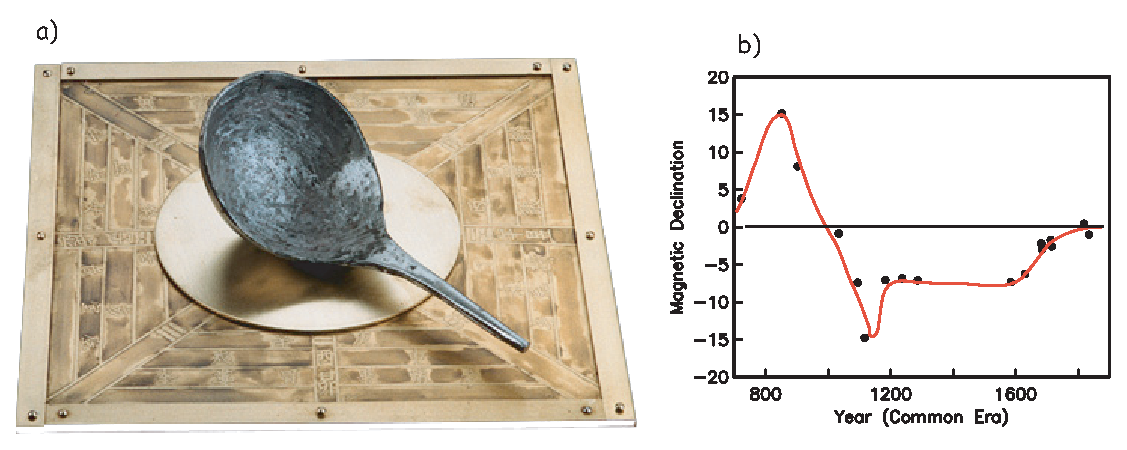
\includegraphics[width=14 cm]{EPSfiles/chinesecompass.eps}
\caption{a) A reconstruction  (Wang , 1948) of the south pointing spoon ({\it shao}) used by the Chinese in the first century CE.  [Photo of Stan Sherer.] ] b) Measurements of magnetic declination made in China from 720 CE to 1829.   [Data quoted  in Smith and Needham, 1967.] }
\label{fig:spoon}
\end{figure}\nocite{wang48}\nocite{smith67}
\eject
To answer some of the questions just raised, we need measurements of the geomagnetic field.  
  The geomagnetic field changes on frequencies of 10s of microseconds (radio waves) to millions and perhaps billions of years.  Direct observations contribute to our knowledge of field behavior for the last few centuries, but on longer times scales we need to use paleomagnetic and archaeomagnetic techniques.    We will first review what is known from historical measurements of the geomagnetic field.  Then we will turn to what we can glean from accidental records made by archaeological and geological materials.  

\section{Historical measurements}
\label{sect:historical}

The magnetic properties of 
\index{lodestone}
lodestone were already  well known  by the early Greeks.   Aristotle (384-332 BCE)  wrote of the work of Greek philosopher Thales of Miletos (624-546 BCE) in his book on the soul ({\it De Anima}): \begin{quote}
Thales, too, to judge from what is recorded about him, seems to have held the soul to be a motive force, since he said that the magnet has a soul in it because it moves the iron.
\end{quote}
But the earliest compass appears to date  from the first century in China.  Lodestone spoons (see Figure~\ref{fig:spoon}a) were placed on bronze plates, often decorated with images of the Big Dipper and other heavenly images.   These ``south pointers'' were apparently used primarily for  prognostication, geomancy and Feng Shui.   It was not until sometime in the late 14th Century that compasses were used for sea-going navigation in China.

\begin{figure}[h!tb]
%\epsfxsize 10cm
%\centering \epsffile{EPSfiles/halley.eps}
\centering  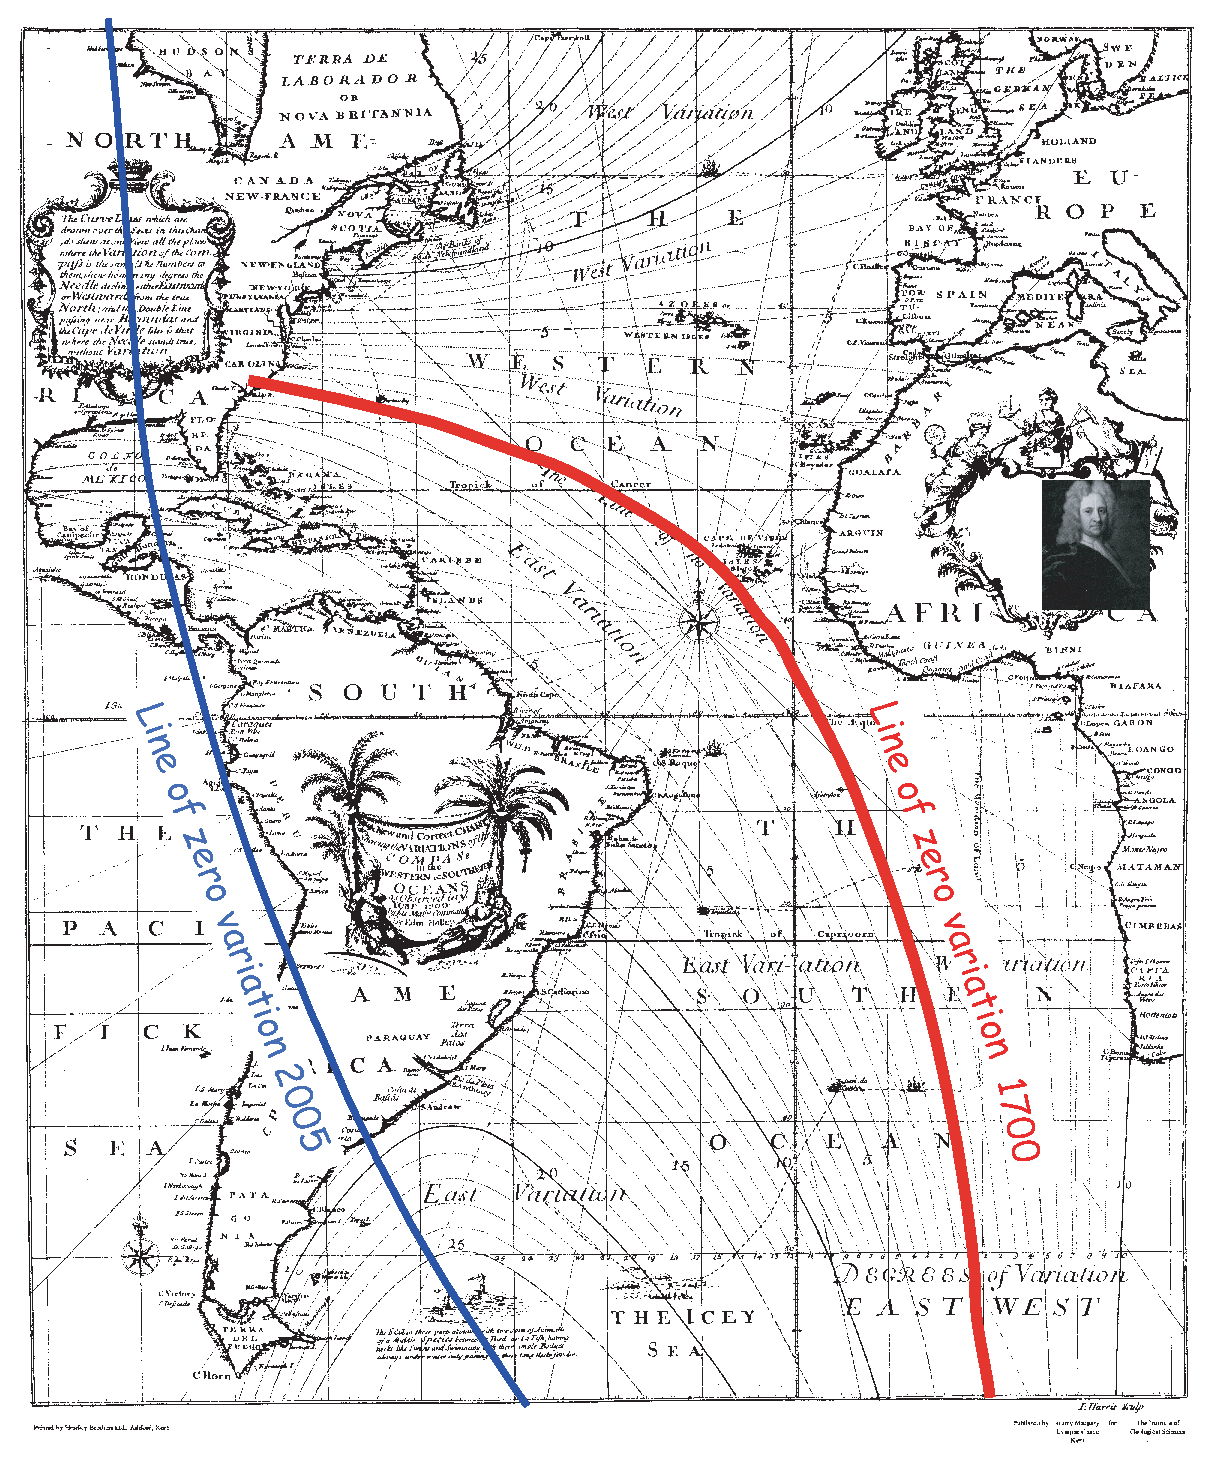
\includegraphics[width=10 cm]{EPSfiles/halley.eps}
\caption{Chart of magnetic declination of Halley. Shown in blue is the line of zero variation from the 2005 IGRF.  [Figure modified from Cook, 2001.]}
\label{fig:halley}
\end{figure}\nocite{cook01}


According to 
\index{Needham, J.}
Needham (1962),  \nocite{needham62} changes in magnetic declination were  discovered in China around 720 CE when the astronomer Yi-Xing measured
\index{magnetic!declination!discovery of}
 magnetic declination (see Figure~\ref{fig:spoon}b).   The compass arrived in Europe some time in the 12$^{th}$ century.  Magnets and compasses were discussed in a letter (Epistola)  by 
 \index{Perigrinus, P.}
Petrus Peregrinus written in 1269 (finally printed in 1558).  Apparently the idea of declination did not accompany the compass. The deviation of magnetic north from true north  was not  rediscovered by Europeans until the early 1400s.  Europeans began to make systematic measurements of declination in the early 1500s.    Magnetic inclination was discovered in the mid-1500s in Europe.

\index{Gilbert, W.}
Gilbert (1600) noted variations in field strength with latitude based on the sluggishness or rapidity with which a compass settled on the magnetic direction.    Magnetic intensity was first measured quantitatively  in the late 1700s by French scientist Robert 
\index{de Paul, R.}
de Paul, although all records were lost in a ship wreck.  The expedition sent to search for the lost ship made several measurements,  using the    period of oscillation $T$ of a vertical dip needle with magnetic moment $m$ and moment of inertia $I$.  These are related to $B$ by: 

$$
T = 2 \pi  \sqrt {{ I \over {mB} }}.
$$
 \noindent
These measurements supported Gilbert's observation that the intensity of the field increases away from the equator.  

The internal origin of the magnetic field was discovered by Gilbert in 1546 who made a systematic study of the magnets and the Earth's magnetic field, published in 1600.   While aware of deviations of magnetic declination from true north, Gilbert thought that the field was unchanging in time.  In 1634  Gellibrand  compared declination measurements made in London over a period of some 50 years and concluded that the geomagnetic field changes.  Thus Europeans discovered secular variation of the magnetic field in 1634, nearly a millenium after the Chinese.  


\begin{figure}[h!tb]
%\epsfxsize 14cm
%\centering \epsffile{EPSfiles/gufm1.eps}
\centering  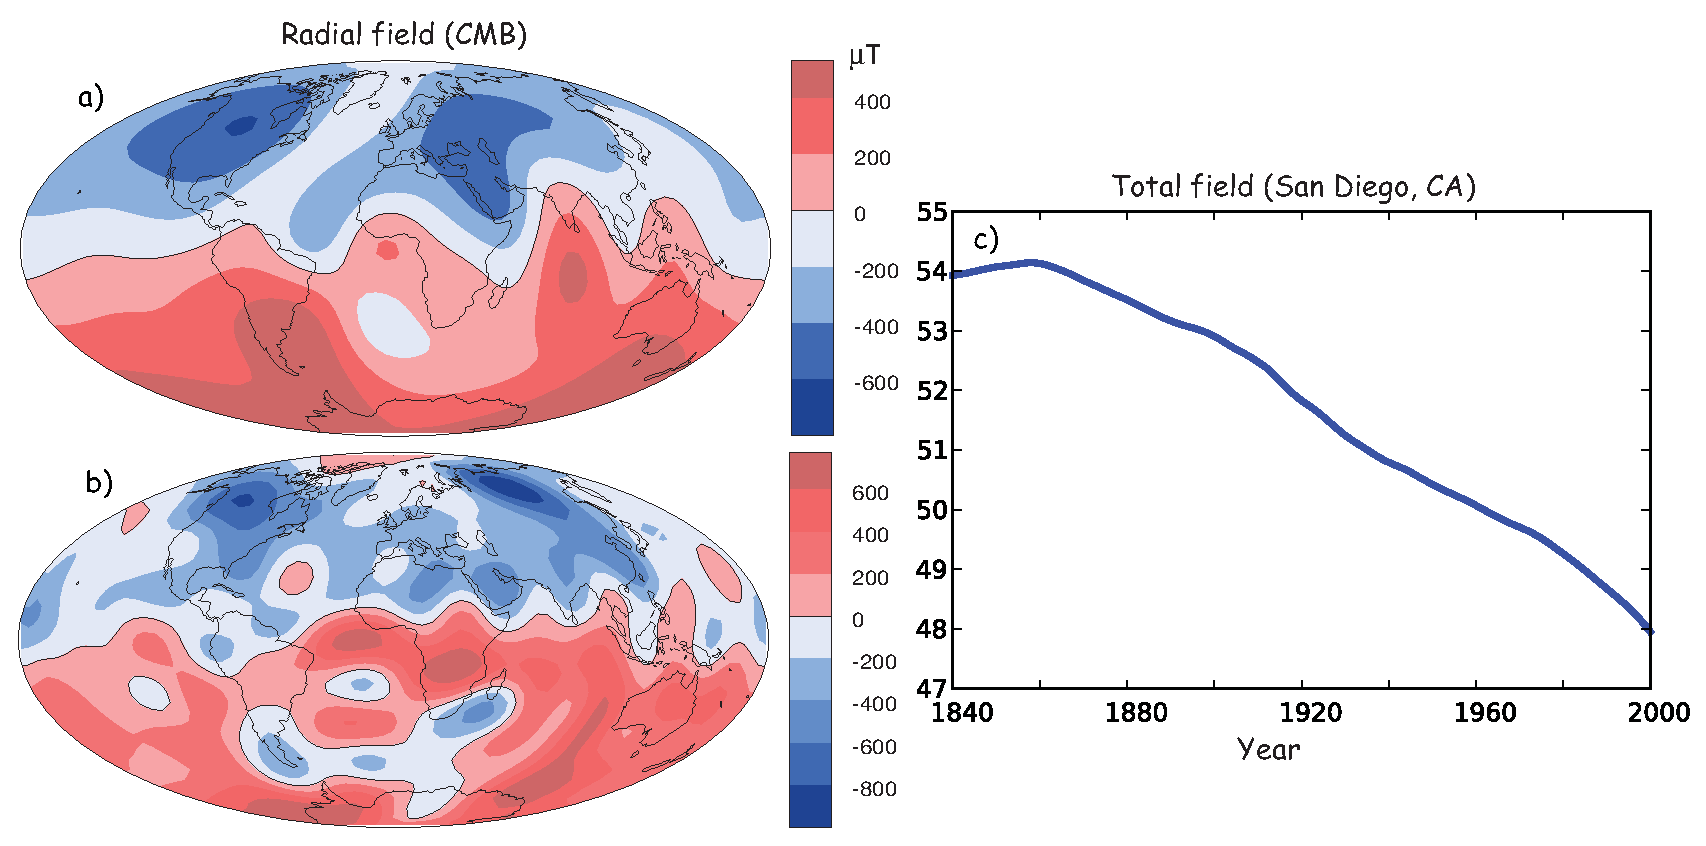
\includegraphics[width=14 cm]{EPSfiles/gufm1.eps}
\caption{Maps of the strength of the radial magnetic field at the core mantle boundary from the {\bf GUFM1} secular variation model of  Jackson et al., (2000).  a) For 1600 CE.  b) For  1990.   c) Field strength in  San Diego, CA evaluated from the {\bf GUFM1} model.}  
\label{fig:gufm1}
\end{figure}  


Captain 
\index{Halley, E.}%
Edmond Halley  carried out  scientific exploration at sea with the expeditions of the Pink Paramore (1698-1701).  He produced the first geomagnetic chart (Figure~\ref{fig:halley}) sometime between 1700 and 1702 (see Reeves, 1918).   \nocite{reeves18}  Halley noticed that some geomagnetic features appeared to be moving to the west, a phenomenon known as {\it westward drift}.  Compare for example the ``line of no variation'' in Figure~\ref{fig:halley} with the line of zero declination from the IGRF of 2005.  It has moved significantly to the west in the equatorial and southern Atlantic realms.  


\index{Gauss, K.F.}
Gauss provided the mathematical framework we use today for dealing with geomagnetic data when he derived the spherical harmonic expression for the geomagnetic potential field (see Chapter  2).  The first such analysis (done in 1835) was based on 84 data points evaluated on an evenly spaced grid from isomagnetic charts of  the magnetic field elements available at the time.  






\begin{figure}[htb]
%\epsfxsize 11cm
%\centering \epsffile{EPSfiles/psvmod.eps}
\centering  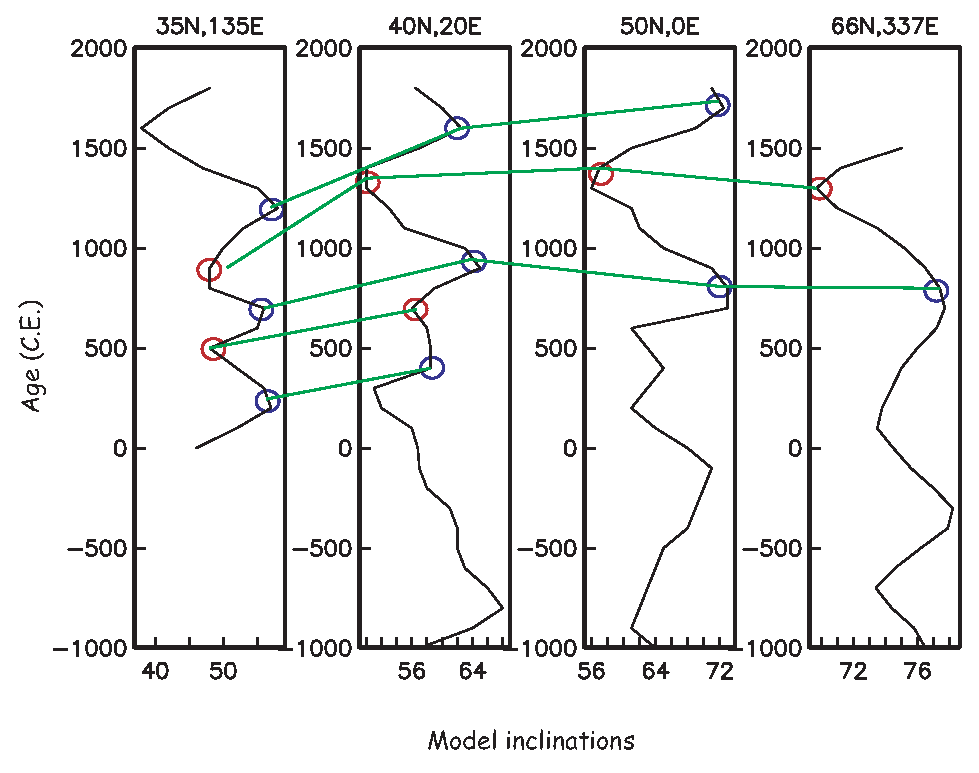
\includegraphics[width=11 cm]{EPSfiles/psvmod}
\caption{Inclinations evaluated at 100 year intervals from the PSVMOD1.0 of Constable et al. (2000) for selected records.  These are plotted from East to West.  Maxima and minima are noted.  Westward drift would imply that these correlated features would ``rise'' to the right.}
\label{fig:psvmod}
\end{figure}




Fastforwarding to the current  millenium, we find researchers still poring over these centuries old measurements.    These ship's logs contain a huge treasure trove of measurements of declination and sometimes inclination since the 16th century.  Such data form the basis for the 
\index{Field models!GUFM1}
{\it GUFM1}  geomagnetic field model
\index{Jackson, A.}
(Jackson et al.,  2000).    \nocite{jackson00}  The strength of the radial component of the magnetic field inferred for the core mantle boundary at two time intervals in the GUFM1 model  is shown in Figure~\ref{fig:gufm1}.  Compare Figure~\ref{fig:gufm1}b with Figure~\ref{fig:harmonics}a in  Chapter 2 which is the strength of the magnetic field observed at the surface.  There are more so-called\index{flux patches}
{\it  flux patches} (the spots of higher intensity) in Figure~\ref{fig:gufm1}b because the field was evaluated closer to the source (the core), but the general pattern is similar.    The field for 1600,  however, was somewhat different.  The number and positions of the flux patches has changed substantially since then.  Some flux patches, in particular the prominent patch that is now over Africa, have moved  from the Indian ocean, a phenomenon largely responsible for  
\index{westward drift}
{\it westward drift}.   

As already mentioned, observatory measurements of the intensity of the magnetic field are only available since the mid-19th century.  These show that the  large changes in declination and inclination were also accompanied by even more dramatic changes in field strength.  We plot the intensity of the field evaluated from the GUFM1 model  for San Diego, CA, in Figure~\ref{fig:gufm1}c.  If the field continues on its recent trajectory, it will reach zero by the year 2500.  

\section{Archaeo- and paleomagnetic records}
\label{sect:psv}

Historical observations quickly run out as we go back in time.  Prior to 720 CE there are no surviving human measurements.  Yet the average field based on the historical measurements
\index{Jackson, A.}
 (e.g., Jackson et al., 2000) is clearly not  GAD.   To see how observations of the magnetic field such as westward drift, quasi-stationary flux lobes and the degree of  ``GADness'' change through time, we must turn to rock and archaeological materials to give us a picture of the ancient geomagnetic field.  


\subsection{Pioneers in paleomagnetism}

Strongly magnetized rocks (as opposed to the mineral lodestone) had been noticed during the 1700s because of their effect on compass needles, but the fact that certain rocks were magnetized in the direction of the Earth's field was discovered by Delesse in 1849 and Melloni in 1853.   
\index{Folgheraiter, G.}
  Folgheraiter extended the study of fossil magnetizations to the magnetic properties of baked archaeological materials in 1899.    \nocite{folgheraiter1899}
Naturally baked material (heated by lava flows) was studied by 
\index{David, P.}
David (1904) \nocite{david04} and \index{Brunhes, B.}
Brunhes (1906). \nocite{brunhes06}  In the course of their investigations, they discovered materials adjacent to normally magnetized rock  that were magnetized in a direction opposite to the Earth's field.  This first application of the baked contact test led to speculation that the Earth's field had reversed its polarity in the past.   
\index{Mercanton, P.L.} \nocite{mercanton26}
 Mercanton (1926)  argued that the field had reversed polarity because reversely magnetized rocks were found all over the world.   
 \index{Matuyama, M.} \nocite{matuyama29}
 Matuyama (1929)   further supported the argument by demonstrating that all the reversely magnetized rocks in Japan were older than the overlying normally magnetized rocks.   It was not until the combined use of paleomagnetism and K-Ar dating allowed  researchers in the U.S. and Australia (e.g., 
 \index{Cox, A.} \nocite{cox63} \nocite{mcdougall63}
 Cox et al., 1963; 
 \index{McDougall, I.}
 \index{Tarling, D.H.}
 McDougall and Tarling, 1963) to demonstrate the global synchrony of polarity intervals that the scientific community embraced the notion of polarity reversals.  


Sedimentary materials were first used  for the investigation of secular variation   by \index{Johnson, E.A.} 
Johnson et al. (1948) \nocite{johnson48} who measured samples from varved lakes in New England.   Mackereth developed a pneumatic coring device for use in  lakes in 1958, opening the way for studies of the detailed time variations of the magnetic field.  
 
\begin{figure}[htb]
%\epsfxsize 13cm
%\centering \epsffile{EPSfiles/wilsoncreek.eps}
\centering  \includegraphics[width=13 cm]{EPSfiles/wilsoncreek.eps}
\caption{ Paleosecular variation of the magnetic field ($D$ and $I$)
observed in the Wilson Creek section north of Mono Lake.  The inclination expected from a geocentric axial dipole is shown as a dashed line.  The declination is
expected to be zero.  The so-called ``Mono
 Lake'' excursion is
marked. The data are from
 Lund et al. (1988) and represent some 23 kyr of time. }
\label{fig:lund}
\end{figure} \nocite{lund88}



\subsection{The last seven millenia}  

Spherical harmonic models  that push back our understanding of geomagnetic field behavior to times without deliberate, systematic human measurements rely on compilations of archaeomagnetic and paleomagnetic data.  
\index{Constable, C.G.}
Constable et al. (2000)  \nocite{constable00}
assembled a data set of 24 time series of directional data from archaeomagnetic and lake sediment sources evaluated at 100 year intervals 
\index{Field models!PSVMOD1.0}
(PSVMOD1.0). 
 We plot examples of several of the inclination records from East to West in Figure~\ref{fig:psvmod}.  

  These efforts were significantly advanced by the inclusion of archaeological and volcanic data sets which resulted in a series of models of the form 
\index{Field models!ICALSxK.n}
  CALSxK.n  (e.g., Korte and Constable, 2003, 2005).  The name  stands for ``Continuous models of \nocite{korte05}
Archaeomagnetic and Lake Sediment data for the past
x thousand years, version n.     The first model of this series,  CALS3K.1 
\index{Korte, M.}
\index{Constable, C.G.}
(Korte and Constable, 2003) \nocite{korte03} included no intensity information, while a more recent version, CALS7k.2,  relies on the data compilation of 
\index{Korte, M.}
Korte et al. (2005) \nocite{korte05b} including directional and intensity data from archaeological, sedimentary and volcanic sources spanning the last seven millennia.  

The CALS7K.2 model can be used  for a wide range of studies (see 
\index{Korte, M.}
\index{Constable, C.G.}
Korte and Constable, 2008). \nocite{korte08}  For example, we can begin to answer questions  such as the control of the geomagnetic field on production of cosmogenic nuclides, or  millennial scale variability in the geomagnetic dipole.   Geomagnetic field vectors can be predicted for a given place at a given time. Predictions from paleosecular variation ``master curves'' are frequently   used to provide constraints for archaeomagnetic dating (see, e.g., 
\index{Lanos, P.}
Lanos et al., 2005) and more accurate field models of the CALSxK style will improve such constraints considerably.  \nocite{lanos05}  

New data compilations are being published every year (e.g., the
\index{databases!GEOMAGIA50}
 Geomagia50 database of  
 \index{Korhonen, K.}
 Korhonen et al., 2008 and   
 \index{databases!ArchaeoINT}
 ArchaeoInt database of
 \index{Genevey, A.}
  Genevey et al., 2008).   \nocite{korhonen08,genevey08}   With these new comprehensive data collections, improved  models will be constructed for longer time series.  This is a fast moving field, so stay tuned.  


\subsection {Westward drift}

\index{westward drift}
We  mentioned that early workers measuring the secular variation of declination noticed that certain features appeared to move west with time.  A careful look at the data shows that  this tendency is a subtle, probably only locally observed effect.  \index{Yukutake, T.}
Yukutake (1967)\nocite{yukutake67} collected together the data available at the time and marked the occurrences of maxima and minima in both declination and inclination.   Some of these are marked on Figure~\ref{fig:psvmod} as examples.  Yukutake then plotted these maxima and minima as a function of age and longitude of the observation site.  The data appeared to suggest that the features moved westward at a rate of about a half a degree per year.  This would mean that the maxima and minima on Figure~\ref{fig:psvmod} would rise to the right as they sort of do, but the data are rather unconvincing.  


\begin{figure}[htb]
%\epsfxsize 13cm
%\centering \epsffile{EPSfiles/sint800.eps}
\centering  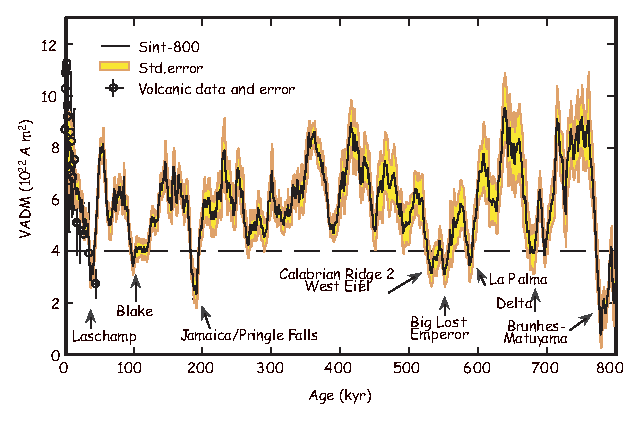
\includegraphics[width=13 cm]{EPSfiles/sint800.eps}
\caption{Stack of relative  paleointensity records from deep sea sediments.  [Figure  modified  from Guyodo and Valet, 1999.] } 
\label{fig:sint800}
\end{figure}\nocite{guyodo99}



\subsection{The more distant past}



For more distant times in the past, accurate chronological constraints become difficult and direct comparison of geomagnetic features globally becomes more difficult.   Field models of the GUFM and CALSxK type which predict geomagnetic field vectors for any place at any time become increasingly more difficult to constrain.  Nonetheless, there are important questions that can be addressed.  


For example: 
\begin{enumerate}
\item  Secular variation over the last few millennia has involved factor of two changes in geomagnetic field strength and directional variability of tens of degrees.  How does the geomagnetic field behave over longer time intervals?  How strong can the field get?  How fast can it change?
\item The geomagnetic field is clearly not entirely dipolar, yet much of paleomagnetic research relies on the assumption that on average the geomagnetic field is that of a geocentric axial dipole. How much time must be averaged for this to be a good approximation?  
\end{enumerate}


  There are two approaches to studying the geomagnetic field in ancient times:  examination of time series from data for which chronological  ordering is known and estimating statistical properties of the paleomagnetic field.      
 In the following sections we will consider first what we have learned from the time series approach and then we will turn to statistical models.    
 
  \begin{figure}[p]
 %\epsfxsize 14.5cm
%\centering \epsffile{EPSfiles/sedpint.eps}
\centering  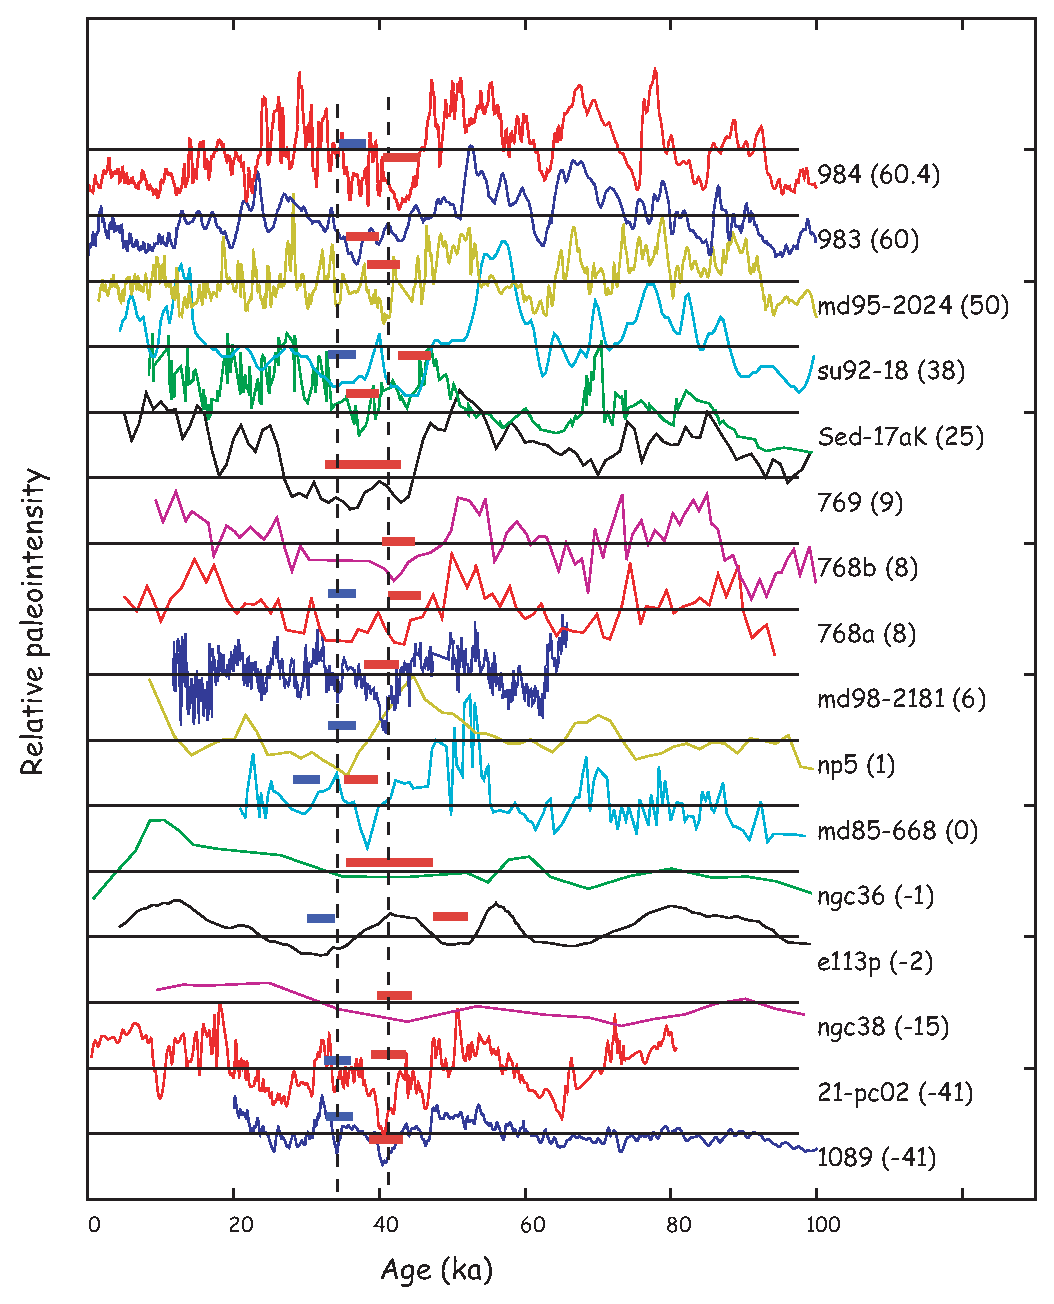
\includegraphics[width=14.5 cm]{EPSfiles/sedpint.eps}
\caption{Relative paleointensity records spanning the last 100 kyr with independent age control based on $\delta^{18}$O.  The solid red bars indicate intensity lows that are possibly related to the  ``Laschamp excursion'' and the blue bars are a later paleointensity low,  referred to as the ``Mono Lake excursion''. [Figure from Tauxe and Yamazaki, 2007.] } 
\label{fig:sedpint}
\end{figure}

 
\section{Time series of paleomagnetic data}   

\subsection{Excursions}

 In Figure~\ref{fig:lund}, we see an example of a detailed record of the geomagnetic field, obtained from dry lake sediments exposed along the shores of Mono Lake in California.     The geomagnetic field oscillated 
 around the  direction expected from a GAD field 
over an interval of some 9 meters.   The amplitude of directional variability is generally contained within about  30$^{\circ}$ of the GAD direction.     At  about 6.75 m, however, the  
field  direction departed drastically from that, achieving a nearly antipodal direction.    This type of behavior is known as a 
\index{geomagnetic!excursions}
{\it geomagnetic excursion}.



  The definition of a geomagnetic excursion is problematic.   The traditional definition identifies magnetic records in which the VGPs are more than 45$^{\circ}$ away from the average pole for that time and place as excursional.      As we shall see in  Section~\ref{sect:psvmods}, the scatter in VGPs may depend on latitude with higher scatter at higher latitudes.         Basing the identification of an excursion on a given VGP cut-off angle then means that more excursions will be identified at higher latitudes.    
  
  
    In a recent review of the phenomenon on excursions,
  \nocite{laj07} 
  \index{Laj, C.}
  \index{Channell, J.E.T.}
Laj and Channell (2007)  advocated that the term be used for features
that represent departures from ``normal'' secular variation,
for which a full polarity reversal has not been
established.  This usage is quite vague, relying on an undefined concept  of what is ``normal''.   They introduced the term {\it microchron} for brief polarity intervals.  These would exhibit fully reversed directions and would presumably be globally oberved.    Other definitions of the term ``excursion'' have been used implicitly.  For example, 
excursions are thought to be accompanied by a decreases in paleointensity (DIPs) (a paleointensity low).   For this reason, some studies (e.g., 
\index{Guyodo, Y.}
\index{Valet, J.-P.}
Guyodo and Valet, 1999) \nocite{guyodo99}  have  identified ``excursions'' based on the occurrence  of paleointensity lows (see Figure~\ref{fig:sint800}).    The rationale for this lies in the fact that most ``deviant'' directions that have paleointensity data associated with them, have ``low'' values (see Section~\ref{sect:trans}).     

\begin{figure}[htb]
%\epsfxsize 10cm
%\centering \epsffile{EPSfiles/919.eps}
\centering  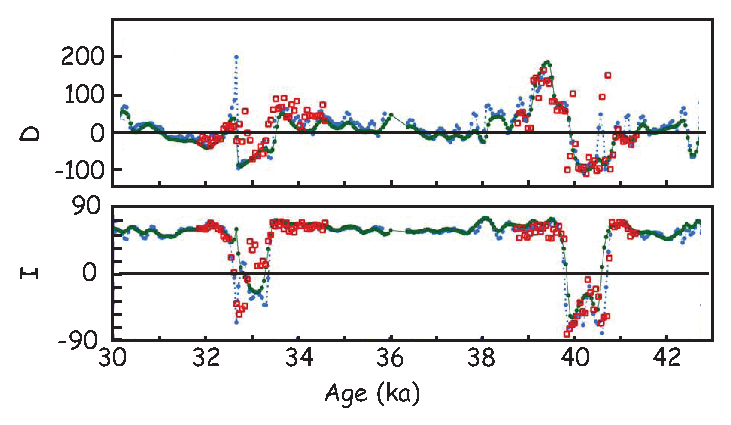
\includegraphics[width=10 cm]{EPSfiles/919.eps}
\caption{Directional data from ODP Site 919.  Declination ($D$) and inclination ($I$) data from continuous core (``u-channel'') measurements  (dark/green closed symbols connected by line), deconvolved u-channel data (closed gray/blue symbols connected by dashed line) and data from 1cc
 discrete samples (open/red squares without connecting line). [Figure redrawm from Channell (2006).] } 
\label{fig:919}
\end{figure}



We name excursions after the place where it was first observed, so the one documented in Figure~\ref{fig:lund} is  known as   the
\index{geomagnetic!excursions!Mono Lake}
{\it Mono Lake excursion}.       This presupposes that the Mono Lake excursion is unique from other excursions requiring a global assessment of excursions and  their ages.    The age of the Mono Lake record has been hotly contested. 
\index{Kent, D.V.}
 Kent et al. (2002) \nocite{kent02}  argue that it is approximately 38-41 ka, which is quite similar to the age of another famous  excursion, the 
 \index{geomagnetic!excursions!Laschamp}
{\it Laschamp excursion}, discovered in volcanics near Laschamp, France (see 
 \index{Bonhommet, N.}
 Bonhommet and
 \index{Z\"ahringer, J.}
  Z\"ahringer, 1969 and references therein; see also 
  \index{Plenier, G.}
  Plenier et al. 2007 for recent review of the Laschamp data). \nocite{bonhommet69}    \nocite{plenier07}   

 Dating sedimentary sequences like the Mono Lake is difficult, but so is dating very young lava flows like the Laschamp volcanics because of the low abundance of radioactive potassium. 
 \index{Zimmerman, S.}
  Zimmerman et al. (2006) weighed in on the issue using relative paleointensity data from the Wilson Creek section \nocite{zimmerman06} (shown in Figure~\ref{fig:lund}) and concluded that the data agree best with relative paleointensity data unequivocally associated with the Laschamp excursion.   
  \index{Cassata, W.S.}
  Cassata et al. (2008) \nocite{cassata08} report new $^{36}$Ar/$^{39}$Ar ages ranging from 31.6$\pm$1.8 ka to 39.1$\pm$4.1 ka  for  a set  of volcanic rocks in New Zealand  from which ``excursional'' directions and low paleointensities  had been obtained
  \index{Shibuya, H.}
   (Shibuya et al., 1992; 
  \index{Cassidy, J.}
  Cassidy, 2006; 
  \index{Mochizuki, N.}
  Mochizuki et al., 2006). \nocite{shibuya92,cassidy06,mochizuki06}   Cassata et al. (2008) claim that there are two excursions represented in these lavas and tie them to the Mono Lake and Laschamp excursions, although there is no volcanic stratigraphy to provide independent proof.  The question as to whether there are in fact two independent excursions is unresolved by these data.  

Resolution of the Mono Lake-Laschamp mystery therefore lies in records with stratigraphic age control.  One such record is the paleointensity proxy record of $^{36}$Cl and $^{10}$Be data in Greenland ice cores (GRIP and GISP cores).    The advantage of ice cores is that not only is the relative chronology straight-forward, layer counting in the ice gives ages that are accurate to within 60 years.  The isotopes $^{36}$Cl and $^{10}$Be are produced in the atmosphere by cosmic ray bombardment which is modulated by the geomagnetic field strength and the strength of the solar wind.  Therefore changes in production rate of these isotopes reflects to a large extent reflect changes in intensity of the field.   The isotopic  data from the Greenland Summit cores were summarized by 
\index{Muscheler, R.}
Muscheler et al. (2005). \nocite{muscheler05}  The $^{10}$Be flux data do not show two peaks, but a single peak centered at approximately 39 ka.   The $^{36}$Cl data, however are less straight-forward.  The data differ in two papers published in the same year on the same core by the same group
\index{Wagner, G.}
 (Wagner et al., 2000a,b). \nocite{wagner00,wagner00b}  One of these has two peaks, centered on $\sim$31 and $\sim$39 ka respectively, while the other has but a single peak at $\sim$39 ka.   

Another way of addressing the Mono Lake-Laschamp dilemma would be to look at the sedimentary relative paleointensity database.  
\index{Tauxe, L.}
\index{Yamazaki, T.}
Tauxe and Yamazaki (2007) compiled nearly all  of the published relative paleointensity records.  \nocite{tauxe07}  Data  with independent $\delta^{18}$O age control spanning the last 100 kyrs are shown in Figure~\ref{fig:sedpint}.  DIPs at around $\sim$40 and $\sim$ 30 ka are marked with red and blue bars.  These have been interpreted as representing  the ``Mono Lake'' and ``Laschamp'' excursional paleointensity lows.  While a few records appear to have both, the evidence is not overwhelming for two globally recorded features.      


Finally, we have the directional records from  sedimentary sequences long enough to record both excursions.    
\index{Channell, J.E.T.}
Channell (2006) \nocite{channell06} published a detailed record with  adequate independent age constraints from oxygen isotopes spanning the 30 to 42 kyr interval of interest (see Figure~\ref{fig:919}).   There are two distinct excursional intervals in this record, one at $\sim$33 ka and the other at $\sim$40 ka.  This core comes from quite close to another core,  SU92-18,  whose relative paleointensity is shown in Figure~\ref{fig:sedpint} and is one of the cores with two distinct paleointensity lows.  

\begin{figure}[htb]
%\epsfxsize 14cm
%\centering \epsffile{EPSfiles/reversals.eps}
\centering  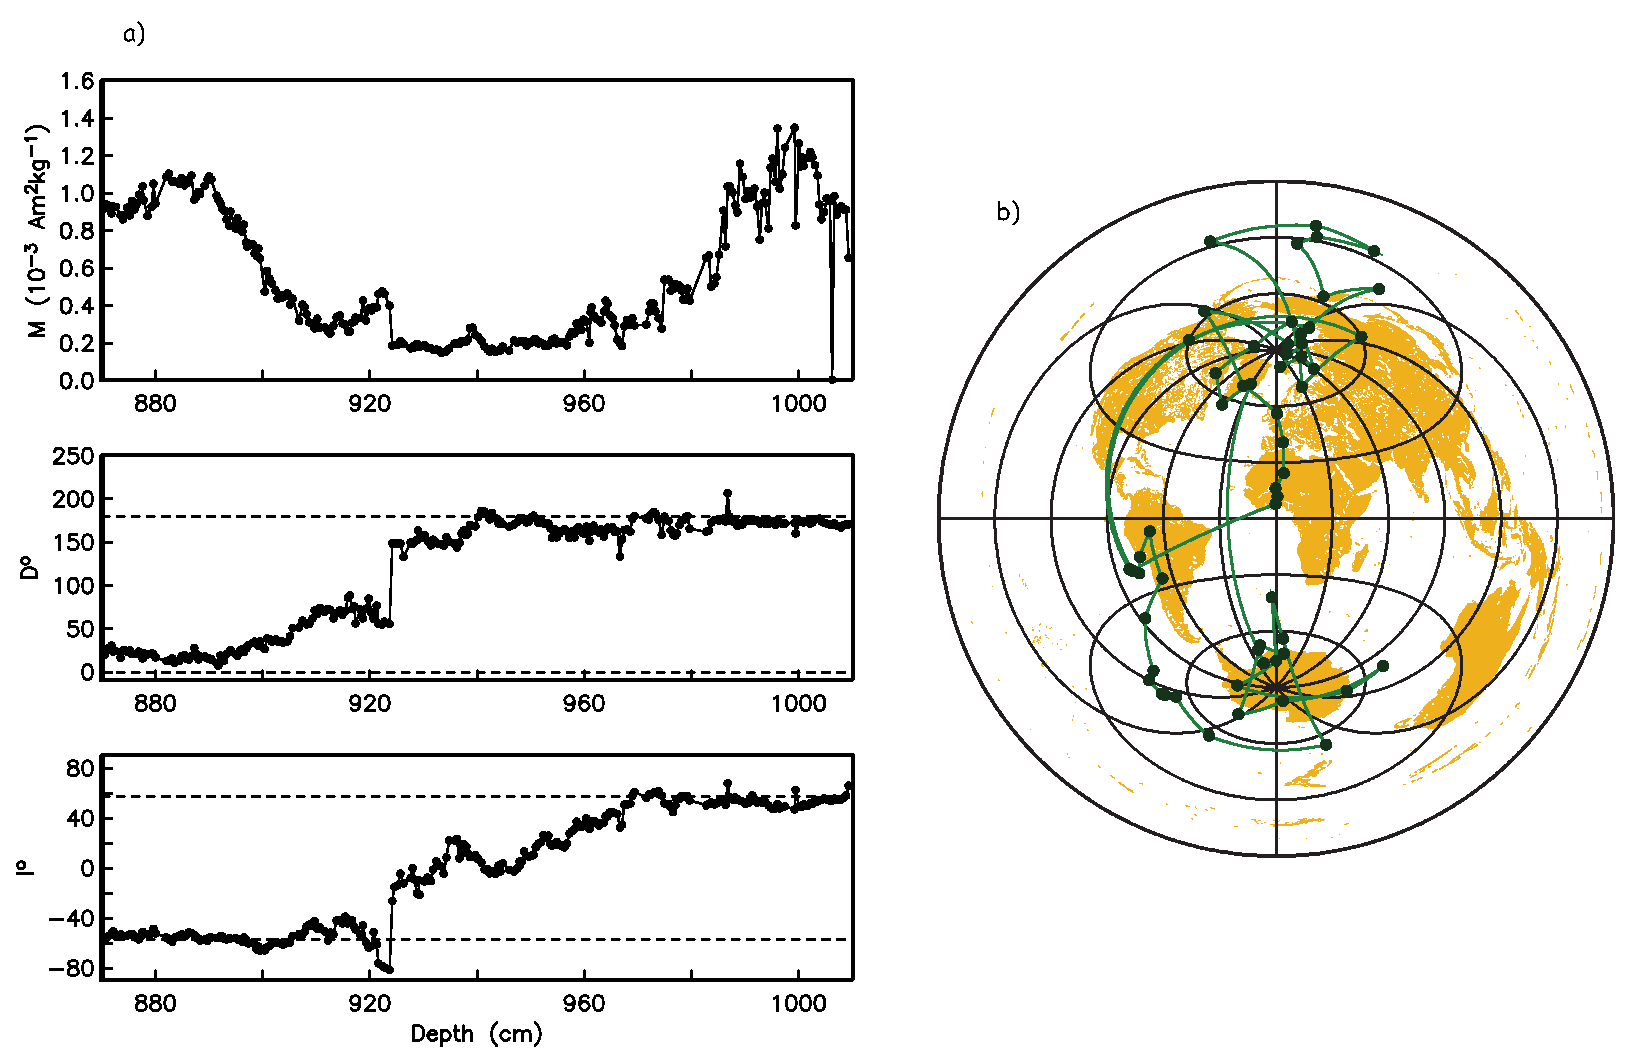
\includegraphics[width=14 cm]{EPSfiles/reversals.eps}
\caption{ a) The lower Jaramillo geomagnetic polarity reversal as recorded in deep sea
sediments from core RC14-14. 
Inclinations and declinations expected from a
normal and reverse GAD field are shown as dashed lines. 
[Data from Clement and Kent, 1984]. b) Record of polarity transition recorded at Steens Mountain. [Data from Camps et al., 1999.]  }
\label{fig:reversals}
\end{figure}


The conclusion from all these different perspectives is that while there may be two excursions at about $\sim$30 and $\sim$40 ka respectively, it is still not clear whether these are global features and which of these the sediments at Mono Lake itself actually recorded.   The conservative interpretation would be  that there is a globally observed  feature with nearly fully reversed directions and low paleointensity values at about $\sim 39 \pm 2$ ka observed in France, California and New Zealand.  Associated low paleomagnetic intensity values at about this time are also observed at in the Greenland ice cores (by $^{10}$Be proxy) and many deep sea sediment cores (Figure~\ref{fig:sedpint}).    This feature should properly be called the ``Laschamp'' and if we adopt the terminology of 
\index{Laj, C.}
\index{Channell, J.E.T.}
Laj and Channell (2007), it would be classified as a microchron.   
It is also clear from the recent literature, that there is no consensus as to what the term  ``excursion'' means.  Laj and Channell (2007) reserve the term for what are essentially local phenomena that do not reach fully antipodal directions.  By this measure,  the feature occasionally observed at about $\sim$ 30 ka would be an excursion.  Because this was first well documented as being a directional feature distinct from the Lashamp in the Irminger Basin (Channell, 2006), perhaps it should be named the Irminger Basin excursion.     



We have examined in detail only a few of the many directional and intensity aberrations that have been called ``excursions'' over the years.   Each has its own history and many may turn out to be as interesting and difficult to pin down as the Mono Lake-Laschamp feature(s).     

\begin{figure}[htb]
%\epsfxsize 14cm
%\centering \epsffile{EPSfiles/vgpspint.eps}
\centering  \includegraphics[width= 14 cm]{EPSfiles/vgpspint.eps}
\caption{ VDM versus VGP latitude from data in the PINT06 database compiled by Tauxe and Yamazaki (2007).  The red triangles are from double heating  experiments with pTRM checks (see Chapter 10).  b) Plot of transitional VGPs (blue dots) from the TRANS data base (McElhinny and Lock, 1996). No selection criteria were applied.  c) Shear wave velocity SB448 model of Masters et al. (2000) evaluated at 2770 km (core mantle boundary region).  There is a fast (cold) ring around the Pacific, presumably from the influence of subducted slabs.   }
\label{fig:vgpspint}
\end{figure}
\nocite{tauxe07,mcelhinny96,masters00}

\subsection{Reversals}
\label{sect:trans}


When viewed over sufficient time, the geomagnetic field 
reverses its polarity, by which we mean
that  the sign of the axial dipole term ($g_1^0$) changes.
An example of a paleomagnetic record of a 
\index{geomagnetic!polarity!reversal}
{\it polarity reversal}  is shown in
Figure~\ref{fig:reversals}a 
\index{Clement, B.M.}
\index{Kent, D.V.}
(Clement and Kent, 1984).  \nocite{clement84}
The intensity of the magnetic field appears to drop to
approximately 10\% of its average value and the directions migrate from
one pole to the other over a period of several thousand years.   When the polarity is the same as the present polarity it is said to be {\it
normal}.
When it is in the opposite state, it is said to be
{\it reverse}.   The duration of the reversal process also appears to be a function of latitude
\index{Clement, B.M.} \nocite{clement04}
 (Clement, 2004).



The details of what happens during a polarity reversal are still rather unclear because they occur so quickly, geologically speaking.   Some high resolution sedimentary records are like that shown in Figure~\ref{fig:reversals} whereby there is an orderly progression from one polarity to the other.  However, a  polarity transition captured by rapidly erupted lava flows records  a more complex picture (see Figure~\ref{fig:reversals}b).   There are a few conclusions we can draw however:  1) they occur quickly and 2) they are always associated with low geomagnetic intensities (see Figure~\ref{fig:vgpspint}a).    

A more controversial observation about directions in extrema was first pointed out by Clement (1991); when mapped to VGP positions, they plot in preferred longitudinal swaths (see Figure~\ref{fig:vgpspint}b).  These swaths are seen in many data sets, but can be made to disappear when certain criteria are applied (e.g., Pr\'evot and Camps, 1993).  The intriguing thing about the swaths is that they appear to coincide with the shear velocity anomalies in the lowermost mantle suggesting some control of the temperature structure near the core mantle boundary on structure of the paleomagnetic field  (see Figure~\ref{fig:vgpspint}c).   Whether or not the swaths exist has been debated ever since they were first observed.  



\begin{figure}[htb]
%\epsfxsize 11cm
%\centering \epsffile{EPSfiles/gpts.eps}
\centering  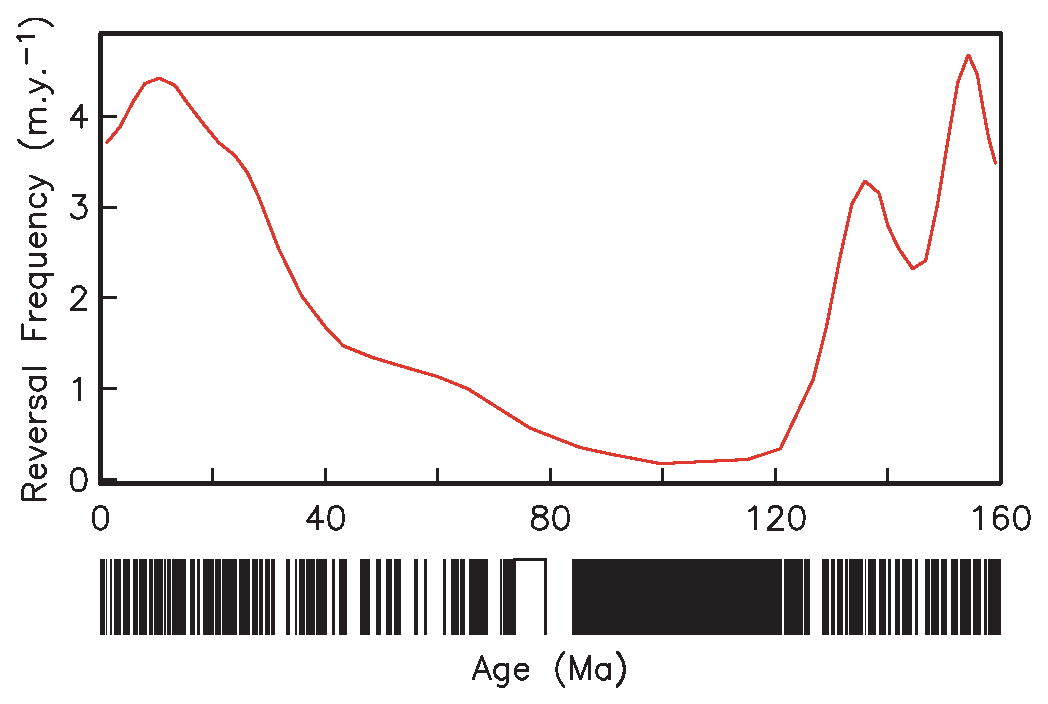
\includegraphics[width=11 cm]{EPSfiles/gpts.eps}
\caption {Barcode: 
The Geomagnetic Polarity Time Scale (GPTS) for the last 160 Ma (Berggren et al., 1995; Gradstein et al., 1995).  Line traces the  reversal
frequency (number of reversals in a four million year interval) estimated by Constable (2003).}
\label{fig:longterm}
\end{figure}



 On average, the field spends about half its time in each polarity state,  
and only a tiny fraction (1-2\%) of the time in an intermediate state.
Rocks of both polarities have been documented from early in the Earth's 
history (at least since the late Archean, see Strik et al. 2003), although the frequency of reversal has changed
considerably through time (see
Opdyke and Channell, 1996    and Merrill et al., 1996).


\section{Geomagnetic polarity time scale -- a first look}

A list of  dates of past geomagnetic polarity reversals is known as a
\index{geomagnetic!polarity!time scale}
 {\it geomagnetic polarity time scale} (GPTS).   How the time scale is calibrated is discussed in the next chapter.  For now we will just take it as a given.  In Figure~\ref{fig:longterm} we show the polarity history from the
marine magnetic anomaly template.
The details of the history of reversals for times older
than the oldest sea floor magnetic anomaly record (about 160 Ma)
are sketchy, but will eventually be
 documented using sedimentary records of the magnetic field (see e.g., 
Kent and Olsen, 1999).   


Examination of the reversal history shown in Figure~\ref{fig:longterm}
suggests that reversals occur at apparently random intervals without a
predictable pattern.  Furthermore, the frequency of reversals appears
to change (see for example,
Constable, 2003).
Above the polarity history in 
Figure~\ref{fig:longterm}, we plot the reversal frequency estimated by 
\index{Constable, C.G.}
Constable (2003). \nocite{constable03}   The reversal
frequency is relatively high in the interval 124-150 Ma, but appears
to drop gradually to zero at the beginning of the so-called Cretaceous
Normal Superchron (CNS), a period of some 38 Myr in which no (or very few)
reversals occurred. Since the end of the CNS at about 83  Ma, the
frequency of reversals has increased to the present average rate of
about four per million years.  


\begin{figure}[htb]
%\epsfxsize 10cm
%\centering \epsffile{EPSfiles/hk02.eps}
\centering  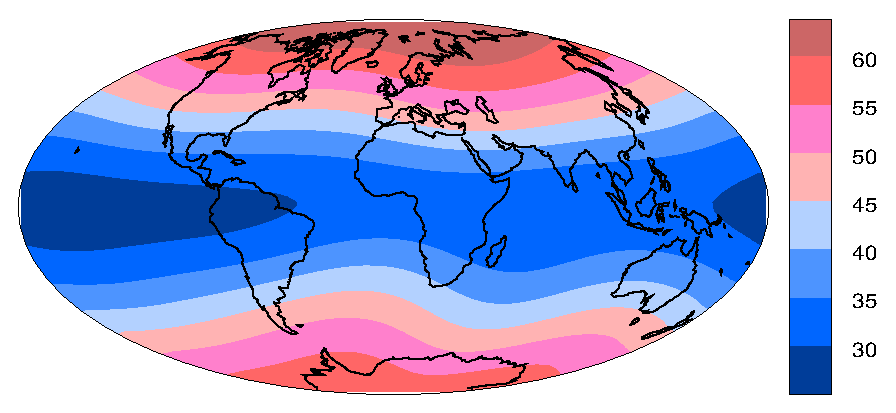
\includegraphics[width=10 cm]{EPSfiles/hk02.eps}
\caption{Time averaged intensity of the geomagnetic field.  [Model  of  Hatakeyama and Kono.  2002.] }
\label{fig:taf}
\end{figure}





\section{The time averaged field}


\index{Field models!time averaged field}
In Sections~\ref{sect:historical} and ~\ref{sect:psv}  we reviewed several field models that were time series of full scale spherical harmonic models.  Beyond a certain age  limit, however, there simply are not enough data with sufficient age control and spatial density to constrain a spherical harmonic model.  The approach for longer time scales has been to look at the average magnetic field or the statistical characterization of paleosecular variation data.  We consider here the time averaged field. 

The last five million years has been a focus  for time average field models because the effects of plate motion are small  and there are hundreds of studies to draw from. Data from lava flows from all over the world have been compiled into various databases and analyzed from a variety of view points.  It was recently realized that the data had been compiled using less than optimum criteria and that many more data of higher overall quality may be required for  a robust TAF model to be produced.  Data from the new TAF project are only just becoming available  (e.g., Johnson et al. 2008).  In the mean time, we show a plot of the  TAF model of Hatakayama and Kono (2002) in Figure~\ref{fig:taf}.  Although the field is not perfectly GAD, the flux patches seen in the historical field are nearly erased.  

One of the primary assumptions in many paleomagnetic studies is that the magnetic field, when averaged over sufficient time, averages to that of a GAD field.    This means that if VGPs are averaged from units spanning enough time to average out secular variation, the mean pole is coincident with the spin axis.     Such a pole is called a 
\index{paleomagnetic!pole}
{\it paleomagnetic pole}.  As continents move, they carry with them rock units that retain a record of the spin axis in the continental reference frame, so these poles tend to form swaths called {\it apparent polar wander paths} or APWPs.  We will learn more about APWPs in Chapter 16.  It is worth mentioning here that it is not very well known exactly how much time is required to average out secular variation;  the consensus is that it is more than 400 years but less than 5 million.    Most text books claim that 10$^4$ --10$^5$ years is sufficient.  The minimum number of sampling sites required for a ``good'' average is also poorly constrained.  Conventional wisdom suggests at least ten,   while  (Tauxe et al., 2003) suggest that approximately 100 sites are required to fully sample secular variation.    


\begin{figure}[htb]
%\epsfxsize 14.5cm
%\centering  \epsffile{EPSfiles/tangent.eps}
\centering  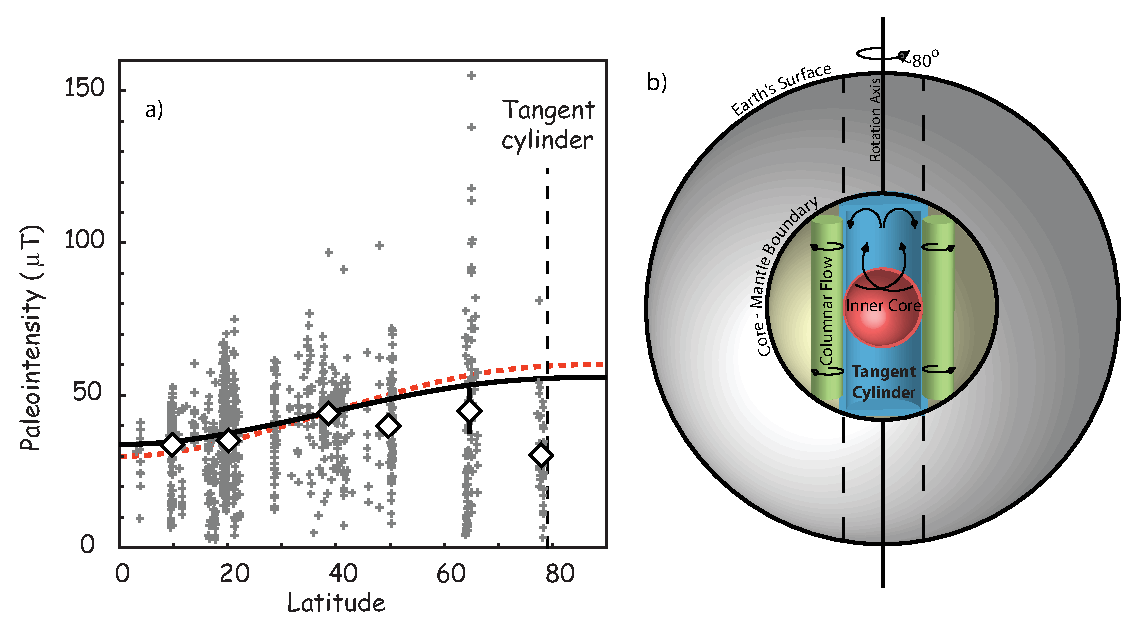
\includegraphics[width=14.5 cm]{EPSfiles/tangent.eps}
\caption{ a)   Paleointensity versus latitude of the Pint06 database (grey crosses) (see Tauxe and
Yamazaki, 2007)  and paleointensity estimates from Lawrence et al. (2009) for data with
ages less than 5 Ma, $d\sigma B \le$ 15 $\mu$T, and $N_{site} \ge$ 2. Mean paleointensity results (diamonds) are calculated for 15$^{\circ}$ latitude bins and errors are shown as 2$\sigma$. The black line
is the longitudinal-averaged intensity for today's field. The vertical dashed line is the
surface expression of the edge of the tangent cylinder.  Southern
hemisphere data have been flipped to the Northern hemisphere. The black line represents
the mean intensity for today's field as defined by the 2005 IGRF model coefficients,
while the red dashed  line represents the intensity associated with a geocentric axial dipole with
a dipole term of 30 $\mu$T.  b)  Illustration of outer core flow regimes. The tangent cylinder is denoted by the blue
 cylinder tangential to the red sphere (inner core). [Figures redrawn from Lawrence et al., 2009.] }
\label{fig:tangent}
\end{figure}
\nocite{lawrence08,tauxe07}
\clearpage

Another aspect of secular variation and the time averaged field is the variation and average strength of the field.  
\index{Tauxe, L.}
\index{Yamazaki, T.}
Tauxe and Yamazaki (2007) \nocite{tauxe07} updated the 
\index{databases!PINT}
PINT03 database of 
\index{Perrin, M.}
\index{Schnepp, E.}
Perrin and Schnepp (2004) \nocite{perrin04}  to include all published paleointensity data through 2006.   We show site-averaged paleointensity estimates
 (grey crosses) derived from the updated paleointensity database  in  Figure~\ref{fig:tangent}a.  We also include the new data from Antarctica of Lawrence et al. (2009).   The only filter for selecting
PINT06 data was that the number of samples had to be at least two and the standard deviation of the site mean intensity had to be less than or equal to 15\%.   Southern hemisphere data are combined with the Northern hemisphere to decrease latitudinal gaps. To reduce the effects of regional variations, the site-level estimates are averaged in 15$^{\circ}$ latitude bins (diamonds) with 95\% confidence levels calculated using a    bootstrap.

One puzzling feature of Figure~\ref{fig:tangent}a is the absence of an increasing trend in the intensity data with latitude. An axial dipole field would have polar intensities twice those expected at the equator, and although for the present field non-axial dipole contributions reduce this gain somewhat (as shown by the solid black line), all conventional wisdom suggests that we would expect the average field strength to increase (double) with latitude. Also shown in Figure~\ref{fig:pint}a (dashed red line)  is field expected from a geocentric dipole with the strength 80 ZAm$^2$.  Neither of these two curves describe the trend in the available data, which if anything suggest {\it weakening} of the field above 65$^{\circ}$.  


\begin{figure}[h!tb]
%\epsfxsize 12.5cm
%\centering \epsffile{EPSfiles/sbg-lava.eps}
\centering  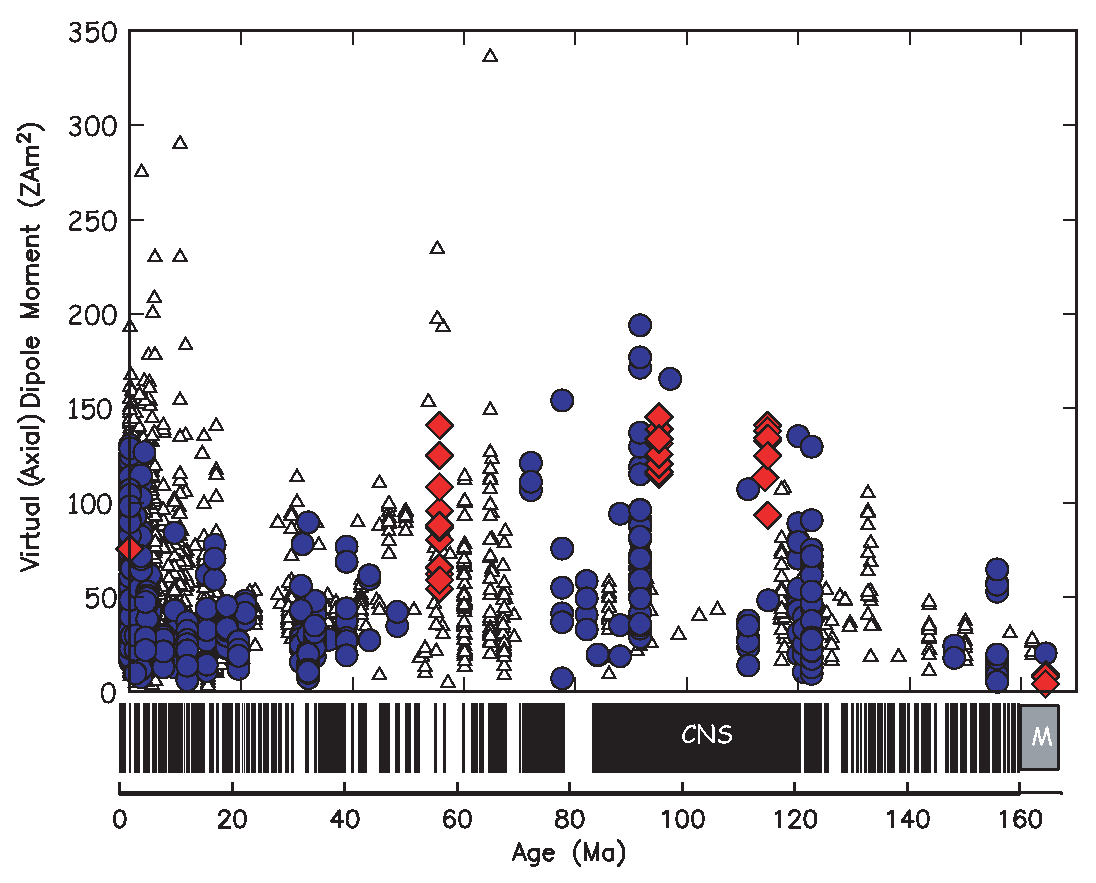
\includegraphics[width=12.5 cm]{EPSfiles/sbg-lava.eps}
\caption{Summary of data  in the PINT06 compilation of Tauxe and Yamazaki (2007) meeting minimum acceptance criteria for last 200 Ma.  Blue dots are submarine basaltic glass data.   Red diamonds are single crystal results.  Triangles are all other data meeting the same consistency criteria ($\sigma < $5\% of mean or $<$5$\mu$T);    At the bottom is the Geomagnetic
Polarity Time Scale showing the Cretaceous Normal Superchron (CNS) and the M-sequence of magnetic anomalies. [Figure from Tauxe and Yamazaki, 2007.]}
\label{fig:pint}
\end{figure}



The apparent trend in intensity might arise from inadequate temporal and geographic sampling of the geomagnetic field (Lawrence et al., 2009). Or,  it is possible that the influence of the  inner core manifests itself in lower average field strengths at and above the cylinder tangent to it (the
\index{tangent cylinder}
 {\it tangent cylinder}).  The geodynamo results from a  complex combination of
physical processes in the fluid outer core  (see, e.g.,
\index{Merrill, R.T.}
Merrill et \nocite{merrill96}
al., 1996).  The influence of the
Coriolis force, combined with the presence of the inner core results 
in a separation of the flow regimes into
two distinct regions bounded by  a cylinder tangent to the inner core, 
 parallel to the spin axis.  (e.g, 
 \index{Aurnou, J.}
 Aurnou et al., 2003; see Figure 
~\ref{fig:tangent}b). 	\nocite{aurnou03}   The spin of the Earth  tends to generate
columnar convection in the region outside the tangent cylinder, while 
inside,    the convection tends to be 
more 3-dimensional
\index{Busse, F.H.}
(Busse, 1983).  \nocite{busse83}  It is possible that the flow regime inside the tangent cylinder results in a depressed field strength observed at high latitude.   












\section{Long term changes in paleointensity}

  We
plot  a compilation of paleointensity  data since the Jurassic in
Figure~\ref{fig:pint}, from Tauxe and Yamazaki (2007).  
Early compilations suggested that much of the Mesozoic  had a rather low field intensity (the 
\index{Mesozoic dipole low}
{\it Mesozoic dipole low} of 
\index{Pr\'evot, M.}
Pr\'evot et al., 1990) \nocite{prevot90}
 with an apparent average intensity of about 25\% of  the 
present field  which is $\sim$ 80  ZAm$^2$.  The more recent compilation of high
quality paleointensity data by 
Tauxe and Yamazaki (2007) shows that the Cenozoic
also had a moderate field, suggesting that the Mesozoic ``dipole
low'' is probably a common state of the geomagnetic field, with
anomalously high values occurring in the latter part of the Cretaceous and early
Cenozoic and during the last few thousand years.  



\begin{figure}[htb]
%\epsfxsize 14cm
%\centering \epsffile{EPSfiles/psvrl.eps}
\centering  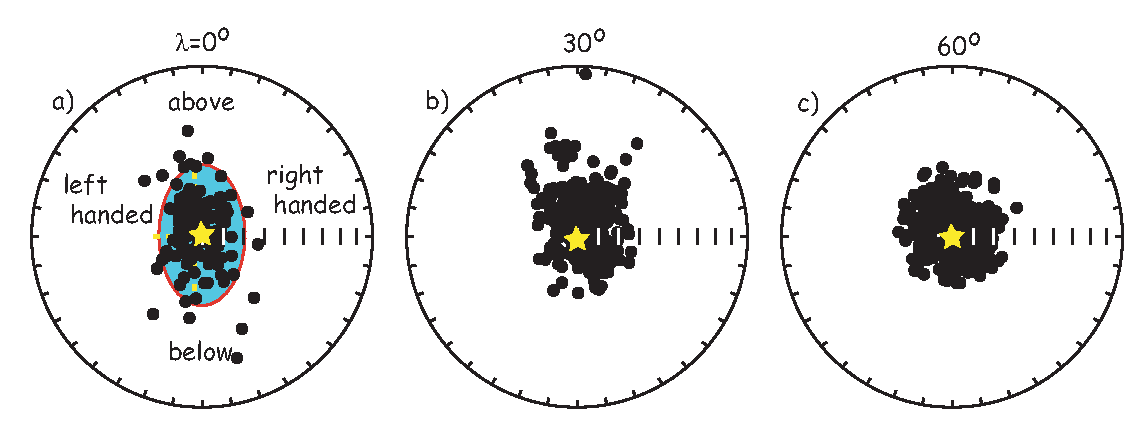
\includegraphics[width=14 cm]{EPSfiles/psvrl.eps}
\caption{a) Paleomagnetic directions from the PSVRL database (see  McElhinny and McFadden, 1997) compiled for latitude band 0-5$^{\circ}$ (N\&S).  Antipodes of reverse directions are used.  The expected direction is at the star at the center of the equal area projection.  Directions in the upper (lower) half are above (below) those expected and those to the right (left) are right-handed (left-handed).  The red ellipse illustrates the elongation $E$ of the directional data where $E$ is the ratio of the eigenvalues along the maximum and minimum axes (here vertical and E-W respectively).   b) Same as a) but for 25-35$^{\circ}$  (N\&S) latitude band.  c) Same as a) but for 55-65$^{\circ}$  (N\&S) latitude band. [Figures redrawn from Tauxe and Kent, 2004.]
   }
\label{fig:psvrl}
\end{figure}

\nocite{tauxe04}

\begin{figure}[htb]
%\epsfxsize 14cm
%\centering \epsffile{EPSfiles/bell.eps}
\centering  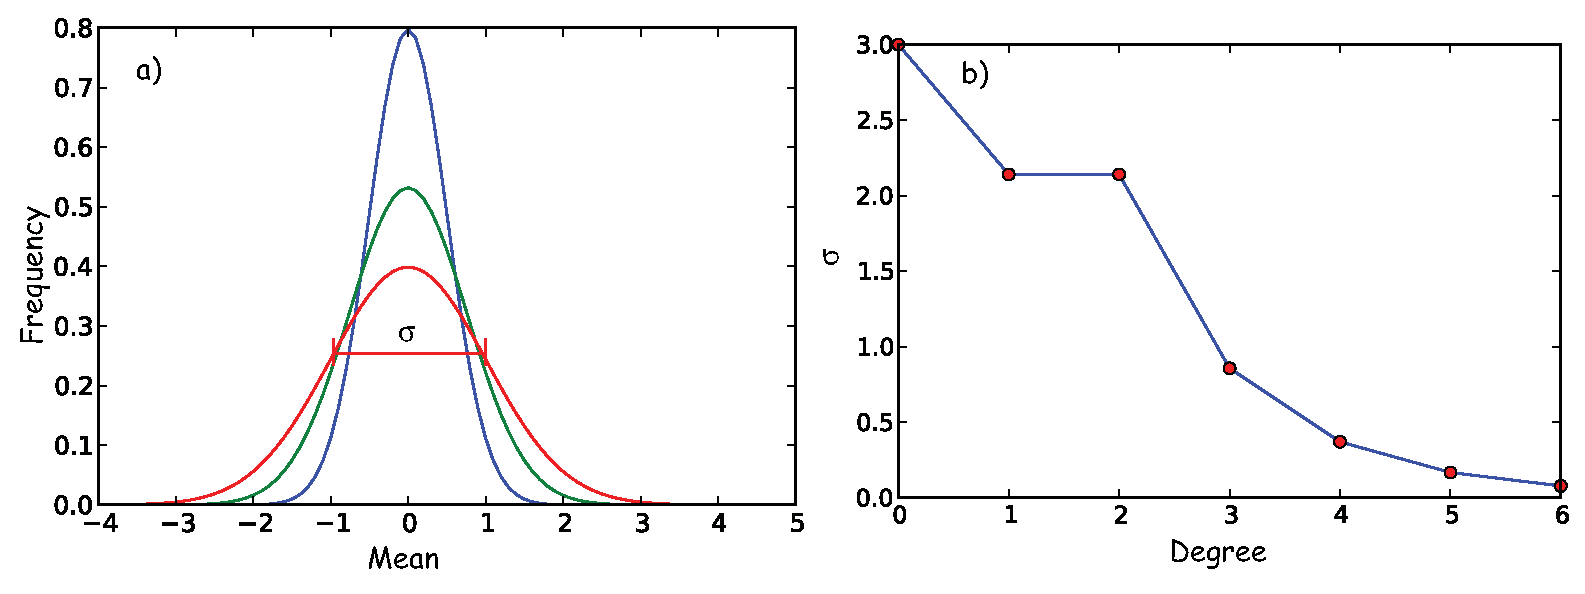
\includegraphics[width=14 cm]{EPSfiles/bell.eps}
\caption{a) Illustration of a normal distribution with varying standard deviations.  b) Variation of standard deviation $\sigma$ as a function of spherical harmonic degree $l$ in the CP88 model. }
\label{fig:bell}
\end{figure}


\section{Statistical models of paleosecular variation}
\label{sect:psvmods}


\index{Field models!statistical}
 From studies of the time averaged field  it seems that, at least for the last five million years, the field has been dominantly that of a geocentric axial dipole (GAD).    At any particular instant in time, however, there will be significant deviations owing to the non-axial dipole contributions.  This, combined with distortions in the recording process (some of which were discussed in Chapter  5) and decreasing preservation of rocks with increasing age makes evaluating the GAD hypothesis increasingly difficult as we go back in time.     
 
 
 
There has been considerable effort in collecting the data relevant to describing the statistical character of the geomagnetic field over time.  Selected results from one  such collection (that of McElhinny and McFadden, 1997; MM97) are shown in Figure~\ref{fig:psvrl}.  Directions from lava flows less than five million years old from particular latitudinal bands are plotted with respect to the expected GAD direction at that particular latitude ($D',I'$ from Chapter 2).     

Several things are worth mentioning about the data in Figure~\ref{fig:psvrl}.  First, it appears that the equatorial data are more elongate than those from higher latitudes (something we mentioned in Chapter  12).  The
\index{elongation}
elongation parameter $E$ can be used to quantify this and is the $\tau_2/\tau_3$ ratio where $\tau_i$ are the eigenvalues of the orientation matrix Appendix~\ref{app:eigen}).  Secondly, the scatter in the directional data seems to go down with increasing latitude.   Thirdly, when the directions are converted to VGPs, the dispersion in VGPs tends to increase with latitude.  

Before we begin a quick tour of PSV models, we must introduce the concept of
\index{virtual!geomagnetic pole!scatter of}
 VGP scatter and briefly explain how it has been calculated.   
VGP scatter is quantified  by the parameter $S_p$  (e.g., {{\it} Cox} 1969), defined   as:
\begin{equation}
S_p^2 = (N -1)^{-1} \sum_{i=1}^N (\Delta_i)^2,
\label{eq:Sp}
\end{equation}
\noindent where $N$ is the number of observations and $\Delta_i$ is the angle between the $i^{th}$ VGP and the spin axis.  

 Ideally, one would use all the paleomagnetic data available, but we encounter two problems with this approach. First, some directions are better determined while others have significant within site scatter resulting from sampling or experimental errors (or lightning strikes!).   Secondly, the interest of the paleomagnetic community in unusual field states (reversals and excursions) has resulted in their over-representation  in the published literature. 



To address the issue of within site scatter,   some studies use a cutoff for $\kappa$ or $\alpha_{95}$ for inclusion in the calculation, while others adjust the value of $S_p$ to account for the within site scatter $S_w$.   
\index{McElhinny, M.W.}
\index{McFadden, P.L.}
McElhinny and McFadden (1997) \nocite{mcelhinny97} defined a parameter $S_f$:

\begin{equation}
S_f^2 = S_p^2 - (S_w^2/\bar n),
\label{eq:Sf}
\end{equation}

\noindent where  $\bar n$ is the average number of samples per site.   

To address the over-representation of unusual field states in the data base, 
some data compilations have used a fixed cutoff for VGP latitude.  For example, the MM97 database culled data with VGP latitudes at 45$^{\circ}$  away from the poles.    The latitudinal dependence of $S_p$ means that a fixed cutoff  biases against the more scattered data collected at higher latitude.  This bias results in a rather peculiar distribution of directions for the high latitude sites (Figure~\ref{fig:psvrl}c).    In an attempt to compensate for this problem,   Vandamme (1994) proposed a variable VGP cutoff \nocite{vandamme94}.  
  The Vandamme cutoff ($A$) is found using a recursive method such that $A = 1.8 S' +5^{\circ}$, where $S'$ is the value of $S_p$ for the trimmed data set.  



Most early modeling efforts by the paleomagnetic community focussed on explaining the variable scatter in directions and VGPs with latitude (see review by 
\index{Tauxe, L.}
Tauxe et al., 2008).  \nocite{tauxe08}
The first model of 
secular variation of the Earth's magnetic field is the 
\index{Field models!dipole wobble}
{\it dipole wobble}  model of \index{Creer, K.M.}
Creer et al. (1959).  \nocite{creer59}This has become known as  Model  B 
\index{Irving, E.A.}
\index{Ward, M.A.}
 (Irving and Ward (1963).  \nocite{irving63}   Dipole wobble (simulated by random variations in the three dipole terms of the spherical harmonic expansion of the geomagnetic field)  produces  \nocite{fisher53} Fisher distributed sets of virtual geomagnetic poles (VGPs).  These are centered around the spin axis.  Because of the non-linear transformation from VGPs to directions (see Chapters 2 and 12), the directions associated with a circularly symmetric set of VGPs  are not generally circular.  

A different PSV model, Model A of 
\index{Irving, E.A.}
\index{Ward, M.A.}
\index{Field models!Model A}
Irving and Ward (1963),  starts from Fisher distributed directional data  modeled by  adding directional perturbations drawn from a uniform distribution  to the expected dipole direction.   The VGP distribution resulting from such a process would be oval at the equator and become more circular toward the poles.   

  \begin{figure}[htb]
%\epsfxsize 13.5cm
%\centering \epsffile{EPSfiles/tk03.eps}
\centering  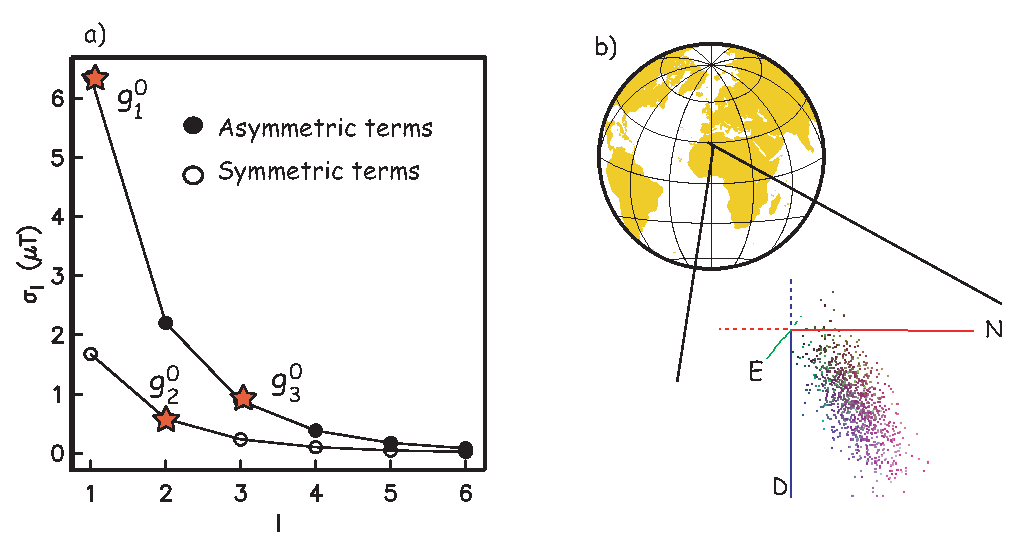
\includegraphics[width=13.5 cm]{EPSfiles/tk03.eps}
\caption{a) Variation of the standard deviation $\sigma_l$ as a function of harmonic degree $l$ for asymmetric and symmetric terms for the statistical field model TK03.GAD.  All terms have zero mean except the axial dipole term.  b)  Estimated  behavior of $S'$ from  the data compilation of McElhinny and McFadden (1997) (circles).   Blue line is the predicted variation of $S'$ from the TK03.GAD model of Tauxe and Kent (2004).  c) 1000 vector endpoints from realizations of model TK03.GAD at 30$^{\circ}$N.   d)    Elongation versus inclination predicted from the TK03.GAD model.  Compilation of data from LIPs of Tauxe et al. (2008).   Crossed open circles are data from large igneous provinces  back through time.  Yemeni traps:  Riisager et al. (2005).   Deccan traps: Vandamme et al. (1991), Vandamme and Courtillot (1992).  Faroe Island basalts: Riisager et al. (2002).  Kerguelen:  Plenier et al. (2002). [Figures from Tauxe and Kent, 2004; Tauxe 2005; Tauxe et al., 2008.]}
\label{fig:tk03}
\end{figure}

\clearpage


\index{Field models!Model G}
Model G of \cite{mcfadden88} modeled the  increasing VGP scatter with latitude by separating the geomagnetic field into the ``dipole'' and ``quadrupole'' families described by \nocite{roberts72} Roberts and Stix (1972).  In the dipole family, the Gauss coefficients  ($g_l^m, h_l^m$)  produce fields that are antisymmetric about the equator (those with $l-m$ odd) while in the quadrupole family, the Gauss coefficients  produce fields that  are symmetric about the equator (those with $l-m$ even).      The antisymmetric terms contribute more strongly to  scatter in VGPs with  latitude than the symmetric terms.   Model G thus has the form:
\begin{equation}
S^2 = (a\lambda)^2 + b^2,
\label{eq:modelG}
\end{equation}



\noindent where $a$ and $b$ are the antisymmetric and symmetric family coefficients,  respectively and $\lambda$ is latitude.  \nocite{mcfadden88} 
\index{McFadden, P.L.}
McElhinny et al. (1997) found that values of $a=0.26\pm0.02$ and $b=11.9\pm 0.7$ provided a good fit to their ``better quality'' dual polarity data set representing the last five million years.  \nocite{mcelhinny97}

Paleosecular variation models of the form of Equation~\ref{eq:modelG} predict average VGP scatter as a function of latitude. 
This is but one of the many interesting and useful observations about the statistical behavior of the magnetic field and  it would be wonderful  if we had a way of predicting for a given latitude the full vector distributions expected from the geomagnetic field.    To find a ``full service''  statistical paleosecular variation model, we begin with  the work of 
\index{Constable, C.G.}
\index{Parker, R.L.}
Constable and Parker (1988;  hereafter CP88).   \nocite{constable88}
\index{Field models!CP88}
  The CP88 statistical paleosecular variation model assumes that the time varying geomagnetic field acts as a ``Giant Gaussian Process'' (GGP) whereby the gauss coefficients (see Chapter 2)   $g_l^m, h_l^m$  (except for the axial dipolar term, $g_1^0$ and in some models also the axial quadrupole term $g_2^0$) have zero mean.  The standard deviations (see Figure~\ref{fig:bell}a)  are a function of degree $l$ and   a fitted parameter $\alpha$ (as in Figure~\ref{fig:bell}b), and, for $l>2$,  follow the formula:
  
  \begin{equation}
{\sigma_l^2 } = { { (c/a)^{2l} \alpha^2}\over {(l+1)(2l+1)} },
\label{eq:sigma1}
\end{equation}

\noindent where $c/a$ is the ratio of the core radius to that of  Earth (0.547).   Many data sets show a persistent offset in equatorial inclinations  at least in reverse polarity data sets, consistent with a small non-zero mean axial quadrupolar term ($\bar g_2^0$).   We are ignoring this effect here because it is in all studies a small term.    
 



In the GAD version of CP88 in which $\bar{g}_2^0=0$, once  the average dipole moment $\bar g_1^0$, its standard deviation $\sigma_1^0$ and $\alpha$ are fixed,  realizations of field models can be created by drawing the gauss coefficients from their respective gaussian distributions.  Geomagnetic vectors can then be calculated for any given location using the usual transformation from the geomagnetic potential equation to geomagnetic elements (see Chapter 2).  


 The principal drawback of the CP88 model is   that it fails to fit the  observed scatter in the paleomagnetic data with latitude. Most of the  subsequent variations on this theme attempted  to address  the VGP scatter problem by introducing more fitted parameters, losing the elegant simplicity of the CP88 model.  

\index{Field models!TK03}
  The most recent model of the statistical paleosecular variation genre is  the TK03.GAD model of  Tauxe and Kent (2004); see also Tauxe et al. (2008). Like CP88.GAD, TK03.GAD has only three parameters:  $\bar g_1^0$ (set to fit a recent estimate for the long term average intensity of the axial dipole as in Figure~\ref{fig:pint}),  $\alpha$ as defined in CP88, but fit to the more recent compilation of directional data of McElhinny and McFadden (1997) and a new paramter $\beta$ which is the ratio of the asymmetric ($l+m$ odd) to the symmetric ($l+m$ even) gauss coefficients for a given $l$.   We show the variation in $\sigma$ with degree for the two families  (asymmetric and symmetric) in Fig.~\ref{fig:tk03}a.    The term $\beta$ allows a much improved fit to the paleomagnetic observations (see Figure~\ref{fig:tk03}b) while the model retains the simplicity of the CP88 model.    Please note that a new generation of models is on the way that will incorporate the vast amount of new data being generated (for a preview of things to come, see Johnson et al., 2008). 
      
 In Fig.~\ref{fig:tk03}c we show the vector end points calculated from 1000 realizations of the model at 30$^{\circ}$N.  The distribution of these vectors predicts what would be observed at that latitude if we had a large number of observations of the geomagnetic field or its paleomagnetic proxies.    
 
 
 Models like TK03 can predict the distribution of geomagnetic field vectors at any location.  These, then, can be compared with the observed paleomagnetic data in order to assess whether the data are consistent with the field model.   The TK03 model was designed to predict values for $S$ in agreement with those observed in the 
 \index{databases!PSVRL}
PSVRL database (see Figure~\ref{fig:tk03}b), but there are other attributes of the field that can be predicted as well.    For example,  while inclination can be calculated from the simple dipole formula (see Chapter 2) for any latitude, the elongation of the directions (e.g., Figure~\ref{fig:psvrl}a) requires a statistical field model.  In fact, because elongation goes down with increasing latitude, while inclination goes up, there is a unique elongation/inclination pair that is consistent with a given statistical field model.  The elongation/inclination trend calculated from the TK03.GAD model is shown in Figure~\ref{fig:tk03}d.  
 

 Data from the last five million years fit the model predictions as it was designed to do, but the model can be tested through time by calculating the elongation/inclination pair for data sets of any age.  The requirements are that the data are referenced to paleo-horizontal,  that the directions represent the ancient geomagnetic field (they are not biased by overprinting, inclination error, etc.), and that there be a sufficient number to represent the statistical variability of the ancient geomagnetic field.   There are not many data sets that satisfy these requirements.  Tauxe et al. (2008) compiled  data sets from ancient large igneous provinces that did:   the Deccan Traps in India (Vandamme et al., 1991, Vandamme and Courtillot, 1992), the Faroe Island basalts (Riisager et al., 2002), and Kerguelen (Plenier et al., 2002).  The elongation/inclination pairs from these data sets are plotted on Figure~\ref{fig:tk03}d for comparison with the model predictions.    It appears that the TK03.GAD model can be used as a guide to the geomagnetic field behavior for at least the Tertiary.   
\vskip 24pt

\noindent SUPPLEMENTAL READINGS:  Tauxe et al. (2008); Johnson et al. (2008).  \nocite{tauxe08,johnson08}


\section{Problems}
{\parindent 0pt  \parskip 12pt
{\bf Problem 1}   

You learned how to use the program {\bf igrf.py} in the problems for Chapter 2. The program uses the official DGRF and IGRF field models since 1945.  A special feature of the program, however, is the use of the GUFM1 coefficients of 
\index{Jackson, A.} \nocite{jackson00}
Jackson et al. (2000) for dates between 1600 and 1945.  

a) Calculate the variation in inclination of the geomagnetic field in Sicily (latitude of 38$^{\circ}$, longitude of 14$^{\circ}$E) between 1600 and 1940 (at 10 year intervals) and make a plot using the {\bf matplotlib} plotting utility.  [There are handy  functions in the {\bf PmagPy} programs and modules ({\bf pmag} and {\bf pmagplotlib} that you are free to call or copy; just do not modify them without renaming them or the {\bf PmagPy} programs won't work right anymore!]   For example, look at {\bf igrf.py} program and  the {\bf pmagplotlib.plotXY} function.

b)  The GUFM1 coefficients were estimated using deliberate, human observations.   An independent dataset is that from lava flows and archaeological artifacts.  These can be searched using the GEOMAGIA web set at \url{http://geomagia.ucsd.edu}.
In the Chapter\_14 data directory in Datafiles (see Chapter 5 for instructions in how to download this) there is a file called {\it geomagia\_sel.txt} with inclination and age data from near the latitude and longitude  of the site examined in a).     Modify your program to plot these data on top of the GUFM predictions.  How do they compare?  

c) Go to the MagIC website (\url{http://earthref.org/MAGIC}) and find out where these data come from.  Are they reliable?  

{\bf Problem 2}


Paleointensity data have been assembled into databases for quite some time.  A recent version of the compilation is in the file {\it PINT08.xls} in the Chapter\_14 data directory.  

a)  Find all the data for the last 10 Myr.  
Select the data that were done with a Thellier double heating type experiment, with pTRM checks (T+) and those that were done with the Shaw method (S).   Plot both sets versus age.  Are there any differences?  

b) Now find all the T+ data that have polarity information for the last 10 Myr.  Separate the data into N, R, and T groups.   Plot these versus age (with different symbols).  Are there any differences?  

{\bf Problem 3}

The dependence of scatter in directions and VGPs on latitude is well known. 

a) Go to the MagIC database website and download the data for one high latitude data set (Lawrence et al., 2009):  \nocite{lawrence08}

 \url{http://earthref.org/MagIC/doi/10.1029/2008GC002072}	

Create a Project Directory and put the file in it.     Use the {\bf QuickMagIC.py} graphical user interface  and cd into your project directory.  Click on ``unpack downloaded txt file'' to extract the data from the txt file.  This will release a number of tab delimited MagIC database formatted files that you can look at using a spreadsheet program.   Read the  documentation at  \url{http://earthref.org/PmagPy/cookbook/#MagIC}  to familiarize yourself with the MagIC database file structure. 

b)  You can read in the site mean data from the {\it pmag\_results.txt} file into a Pandas Dataframe and look them in equal area projection using the {\bf plot\_net} and {\bf plot\_di} functions in the ipmag module of {\bf PmagPy} from within an IPython notebook.   Be sure to get rid of all the blank directional data with the Pandas function dropna. Also, there are study averages, so you need the `individual'  data under the `data type' key (data type is 'i').    Now fish out the VGPs from the same data records and plot them with the ipmag.plot\_vgp function.  To do that, you will need to have Basemap installed and learn how make a simple map (consult the website \url{https://nbviewer.jupyter.org/github/swanson-hysell/2015_Tauxe-et-al_PmagPy_Notebook/blob/master/PmagPy_notebook.ipynb} for help).     As this is a dual polarity data set, first flip the VGPs with negative latitudes to the antipode (subtract 180 from the longitude and take the absolute value of the latitude).  


c)  Write a program that will calculate the $S_p$ VGP scatter statistic from VGPs.   What is $S_p$ of the entire data set?  [Use the antipodes of the reverse data.]  

d)  Now modify your program to calculate $S_p$ as a function of  latitude cutoff, i.e., make an option to exclude VGP latitudes with latitudes more than a specified amount away from the spin axis.    What is the ``best'' latitude cut-off?  

e) A file called {\bf hawaii\_results.txt} is stored in the Chapter\_14 Datafiles directory.  This is a compilation of all the data from Hawaii used in a recent analysis of the time averaged field project by Johnson et al. (2008). \nocite{johnson08}
Repeat problems 2b-d on the Hawaiian data set.  Is there a latitude dependence of $S_p$? 


f) Compare these values of $S_p$  to those predicted by Model G. 



{\bf Problem 4}

a) Use the program {\bf tk03.py} to generate a set of 100 directions for a latitude of 20$^{\circ}$ (the approximate latitude of Hawaii). Save these in a file called {\it hawaii.tk03} and plot them using the program {\bf eqarea.py}.  

b)  Find the present IGRF and GAD directions at 20$^{\circ}$ and -156$^{\circ}$ using the programs {\bf igrf.py} and {\bf dipole\_pinc.py} (or you can use the functions {\bf  ipmag.igrf} and {\bf pmag.pinc(lat)} from inside an IPython notebook).    Rotate the directions in {\it hawaii.tk03}  to the expected GAD direction using the program {\bf di\_rot.py}.  
Plot these rotated directions using {\bf eqarea.py}.  Now rotate the directions extracted from {\it hawaii\_results.txt} in Problem 2e in the same way and plot them in equal area projection.  How do the directions predicted by the PSV field model compare with the data set from Hawaii?  

c) Use the program {\bf goprinc.py} to calculate the eigenparameters of the orientation matrix of the Hawaiian directions (see Chapter 9 and Appendix~\ref{app:eigen}).   What is wrong with either the GAD model or the data set?  


}





